%% History:
% Pavel Tvrdik (26.12.2004)
%  + initial version for PhD Report
%
% Daniel Sykora (27.01.2005)
%
% Michal Valenta (3.12.2008)
% rada zmen ve formatovani (diky M. Duškovi, J. Holubovi a J. Žďárkovi)
% sjednoceni zdrojoveho kodu pro anglickou, ceskou, bakalarskou a diplomovou praci

% One-page layout: (proof-)reading on display
%%%% \documentclass[11pt,oneside,a4paper]{book}
% Two-page layout: final printing
\documentclass[11pt,twoside,a4paper]{book}   
%=-=-=-=-=-=-=-=-=-=-=-=--=%
% The user of this template may find useful to have an alternative to these 
% officially suggested packages:
\usepackage{color}
\usepackage[czech, slovak, english]{babel}
\usepackage[T1]{fontenc} % pouzije EC fonty 
% pripadne pisete-li cesky, pak lze zkusit take:
% \usepackage[OT1]{fontenc} 
\usepackage[utf8]{inputenc}
%=-=-=-=-=-=-=-=-=-=-=-=--=%
% In case of problems with PDF fonts, one may try to uncomment this line:
%\usepackage{lmodern}
%=-=-=-=-=-=-=-=-=-=-=-=--=%
%=-=-=-=-=-=-=-=-=-=-=-=--=%
% Depending on your particular TeX distribution and version of conversion tools 
% (dvips/dvipdf/ps2pdf), some (advanced | desperate) users may prefer to use 
% different settings.
% Please uncomment the following style and use your CSLaTeX (cslatex/pdfcslatex) 
% to process your work. Note however, this file is in UTF-8 and a conversion to 
% your native encoding may be required. Some settings below depend on babel 
% macros and should also be modified. See \selectlanguage \iflanguage.
%\usepackage{czech}  %%%%%\usepackage[T1]{czech} %%%%[IL2] [T1] [OT1]
%=-=-=-=-=-=-=-=-=-=-=-=--=%

%%%%%%%%%%%%%%%%%%%%%%%%%%%%%%%%%%%%%%%
% Styles required in your work follow %
%%%%%%%%%%%%%%%%%%%%%%%%%%%%%%%%%%%%%%%
\usepackage{graphicx}
%\usepackage{indentfirst} %1. odstavec jako v cestine.
\usepackage{amsmath}
\usepackage{lscape}
\usepackage{k336_thesis_macros} % specialni makra pro formatovani DP a BP
 % muzete si vytvorit i sva vlastni v souboru k336_thesis_macros.sty
 % najdete  radu jednoduchych definic, ktere zde ani nejsou pouzity
 % napriklad: 
 % \newcommand{\bfig}{\begin{figure}\begin{center}}
 % \newcommand{\efig}{\end{center}\end{figure}}
 % umoznuje pouzit prikaz \bfig namisto \begin{figure}\begin{center} atd.


%%%%%%%%%%%%%%%%%%%%%%%%%%%%%%%%%%%%%
% Zvolte jednu z moznosti 
% Choose one of the following options
%%%%%%%%%%%%%%%%%%%%%%%%%%%%%%%%%%%%%
\newcommand\TypeOfWork{Diplomová práca} \typeout{Diplomová práce}
% \newcommand\TypeOfWork{Master's Thesis}   \typeout{Master's Thesis} 
%\newcommand\TypeOfWork{Bakalárska práca}  \typeout{Bakalárska práca}
% \newcommand\TypeOfWork{Bachelor's Project}  \typeout{Bachelor's Project}


%%%%%%%%%%%%%%%%%%%%%%%%%%%%%%%%%%%%%
% Zvolte jednu z moznosti 
% Choose one of the following options
%%%%%%%%%%%%%%%%%%%%%%%%%%%%%%%%%%%%%
% nabidky jsou z: http://www.fel.cvut.cz/cz/education/bk/prehled.html

%\newcommand\StudProgram{Elektrotechnika a informatika, dobíhající, Bakalářský}
%\newcommand\StudProgram{Elektrotechnika a informatika, dobíhající, Magisterský}
% \newcommand\StudProgram{Elektrotechnika a informatika, strukturovaný, Bakalářský}
 %\newcommand\StudProgram{Elektrotechnika a informatika, strukturovaný, Navazující magisterský}
\newcommand\StudProgram{Otvorená informatika, Magisterský}
% English study:
% \newcommand\StudProgram{Electrical Engineering and Information Technology}  % bachelor programe
% \newcommand\StudProgram{Electrical Engineering and Information Technology}  %master program


%%%%%%%%%%%%%%%%%%%%%%%%%%%%%%%%%%%%%
% Zvolte jednu z moznosti 
% Choose one of the following options
%%%%%%%%%%%%%%%%%%%%%%%%%%%%%%%%%%%%%
% nabidky jsou z: http://www.fel.cvut.cz/cz/education/bk/prehled.html

%\newcommand\StudBranch{Výpočetní technika}   % pro program EaI bak. (dobihajici i strukt.)
%\newcommand\StudBranch{Výpočetní technika}   % pro prgoram EaI mag. (dobihajici i strukt.)
\newcommand\StudBranch{Softwarové inžinierstvo}            %pro STM
%\newcommand\StudBranch{Web a multimedia}                  % pro STM
%\newcommand\StudBranch{Computer Engineering}              % bachelor programe
%\newcommand\StudBranch{Computer Science and Engineering}  % master programe


%%%%%%%%%%%%%%%%%%%%%%%%%%%%%%%%%%%%%%%%%%%%
% Vyplnte nazev prace, autora a vedouciho
% Set up Work Title, Author and Supervisor
%%%%%%%%%%%%%%%%%%%%%%%%%%%%%%%%%%%%%%%%%%%%

\newcommand\WorkTitle{Veľkoobjemové úložisko emailov}
\newcommand\FirstandFamilyName{Bc. Patrik Lenárt}
\newcommand\Supervisor{Ing. Ján Šedivý, CSc.}



% Pouzijete-li pdflatex, tak je prijemne, kdyz bude mit vase prace
% funkcni odkazy i v pdf formatu
\usepackage[
pdftitle={\WorkTitle},
pdfauthor={\FirstandFamilyName},
bookmarks=true,
colorlinks=true,
breaklinks=true,
urlcolor=red,
citecolor=blue,
linkcolor=blue,
unicode=true,
]
{hyperref}




\begin{document}

%%%%%%%%%%%%%%%%%%%%%%%%%%%%%%%%%%%%%
% Zvolte jednu z moznosti 
% Choose one of the following options
%%%%%%%%%%%%%%%%%%%%%%%%%%%%%%%%%%%%%
\selectlanguage{slovak}
%\selectlanguage{english} 

% prikaz \typeout vypise vyse uvedena nastaveni v prikazovem okne
% pro pohodlne ladeni prace


\iflanguage{slovak}{
	 \typeout{************************************************}
	 \typeout{Zvolený jazyk: slovenčina}
	 \typeout{Typ práce: \TypeOfWork}
	 \typeout{Študijný program: \StudProgram}
	 \typeout{Obor: \StudBranch}
	 \typeout{Meno: \FirstandFamilyName}
	 \typeout{Názov práce: \WorkTitle}
	 \typeout{Vedúci práce: \Supervisor}
	 \typeout{***************************************************}
	 \newcommand\Department{Otvorená informatika}
	 \newcommand\Faculty{Fakulta elektrotechnická}
	 \newcommand\University{České vysoké učení technické v Praze}
	 \newcommand\labelSupervisor{Vedúci práce}
	 \newcommand\labelStudProgram{Študijný program}
	 \newcommand\labelStudBranch{Obor}
}{
	 \typeout{************************************************}
	 \typeout{Language: english}
	 \typeout{Type of Work: \TypeOfWork}
	 \typeout{Study Program: \StudProgram}
	 \typeout{Study Branch: \StudBranch}
	 \typeout{Author: \FirstandFamilyName}
	 \typeout{Title: \WorkTitle}
	 \typeout{Supervisor: \Supervisor}
	 \typeout{***************************************************}
	 \newcommand\Department{Department of Computer Science and Engineering}
	 \newcommand\Faculty{Faculty of Electrical Engineering}
	 \newcommand\University{Czech Technical University in Prague}
	 \newcommand\labelSupervisor{Supervisor}
	 \newcommand\labelStudProgram{Study Programme} 
	 \newcommand\labelStudBranch{Field of Study}
}


%%%%%%%%%%%%%%%%%%%%%%%%%%    Titulni stranka / Title page 

\coverpagestarts

%%%%%%%%%%%%%%%%%%%%%%%%%%%    Podekovani / Acknowledgements 

\acknowledgements
\noindent
%???
%Rád by som poďakoval vedúcemu práce pánovi Ing. Jánovi Šedivému za konzultácie, cenné rady, pripomienky a návrhy, ktoré mi ochotne poskytol počas vypracovávania tejto práce. Tak isto sa chcem poďakovať svojim najbližším, bez ktorých podpory by táto práca nevznikla.


%%%%%%%%%%%%%%%%%%%%%%%%%%%   Prohlaseni / Declaration 

\declaration{V Prahe dňa 1.\,3.\,2011}
%\declaration{In Kořenovice nad Bečvárkou on May 15, 2008}


%%%%%%%%%%%%%%%%%%%%%%%%%%%%    Abstract 
 
\abstractpage
%Simulations of wireless networks play an important role in understanding wireless network properties and following the development of network standards. The aim of this thesis is to research a simulation of a relatively young network, such as standard IEEE 802.15.4, and approximate this model to reality. The model will simulate the antenna’s characteristics, which all devices implementing this standard use for communication. The accuracy of the model will be compared to the real-life measurements and the results will be evaluated.

% Prace v cestine musi krome abstraktu v anglictine obsahovat i
% abstrakt v cestine.
\vglue60mm

\noindent{\Huge \textbf{Abstrakt}}
\vskip 2.75\baselineskip

\noindent
%Simulácie bezdrôtových sieti zohrávajú dôležitú úlohu pri posudzovaní ich vlastností a pri ich následnom vývoji. Cieľom tejto práce bude zrealizovať simuláciu pomerne mladého bezdrôtového štandardu IEEE 802.15.4 a priblížiť model tejto simulácie realite. Model bude využívať charakteristiky antén, ktoré dané zariadenia implementujúce tento štandard využívajú pri svojej vzájomnej komunikácii. Presnosť daného modelu následne overím pomocou meraní, ktoré boli uskutočnené v reálnych podmienkach a zhodnotím dosiahnuté výsledky. 

%Abstrakt práce by měl velmi stručně vystihovat její podstatu. Tedy čím se práce zabývá a co je jejím výsledkem/přínosem.

%%%%%%%%%%%%%%%%%%%%%%%%%%%%%%%%  Obsah / Table of Contents 

\tableofcontents


%%%%%%%%%%%%%%%%%%%%%%%%%%%%%%%  Seznam obrazku / List of Figures 

\listoffigures


%%%%%%%%%%%%%%%%%%%%%%%%%%%%%%%  Seznam tabulek / List of Tables

\listoftables


%**************************************************************

\mainbodystarts
% horizontalní mezera mezi dvema odstavci
%\parskip=5pt
%11.12.2008 parskip + tolerance
\normalfont
\parskip=0.2\baselineskip plus 0.2\baselineskip minus 0.1\baselineskip

% Odsazeni prvniho radku odstavce resi class book (neaplikuje se na prvni 
% odstavce kapitol, sekci, podsekci atd.) Viz usepackage{indentfirst}.
% Chcete-li selektivne zamezit odsazeni 1. radku nektereho odstavce,
% pouzijte prikaz \noindent.

%**************************************************************

% Pro snadnejsi praci s vetsimi texty je rozumne tyto rozdelit
% do samostatnych souboru nejlepe dle kapitol a tyto potom vkladat
% pomoci prikazu \include{jmeno_souboru.tex} nebo \include{jmeno_souboru}.
% Napr.:
% \include{1_uvod}
% \include{2_teorie}
% atd...

%*****************************************************************************
\chapter{Úvod}
%Úvod charakterizující kontext zadání, případně motivace.
S neustálym rozvojom informačných technológií súčasne narastá objem informácií, ktoré je potrebné spracúvať. Tento fakt podnietil vznik databázových systémov, ktoré slúžia na organizáciu, uchovávanie a prácu s veľkým objemom dát. V dnešnej dobe existuje množstvo databázových systémov, ktoré sa navzájom líšia svojou architektúrou, dátovým modelom, výrobcom atď.

Od začiatku sedemdesiatych rokov 20. storočia sú v tejto oblasti dominantou relačné databázové systémy (Relational Database Management Systems). Vďaka neustálemu prudkému rozvoju internetových technológií a rapídnemu rastu dát v digitálnom univerze \cite{digitalUniverse} začínajú byť tieto systémy nepostačujúce. Medzi hlavné faktory pre výber relačného databázového systému doposiaľ patrili výrobca, cena a pod. V dnešnej dobe so vznikom moderných aplikácií (napríklad sociálne siete, dátové sklady, analytické aplikácie a iné), požadujeme od týchto systémov vlastnosti ako vysoká dostupnosť, horizotnálna rozšíriteľnosť a schopnosť pracovať s obrovským objemom dát (petabyte). Novo vznikajúce databázové systémy, spĺňajúce tieto požiadavky sa spoločne označujú pod názvom NoSQL (Not Only SQL). Pri ich výbere je v tomto prípade dôležité porozumenie architektúry, dátového modelu a dát, s ktorými budú tieto systémy pracovať.

Táto práca si kladie za cieľ viacero úloh, ktorými sú pochopenie a popis základných  konceptov, ktoré tieto systémy využívajú, určenie kritérií vďaka ktorým môžeme tieto systémy navzájom porovnávať. Ďalej je úlohou analýzovať a popísať požiadavky pre systém veľkoobjemového úložiska elektronickej pošty, ktorý bude schopný spracovávať milióny emailov. Poslednou úlohou je na základe našich požiadavkov vybrať, čo najlepšie odpovedajúci NoSQL systém a s jeho použitím implementovať prototyp aplikácie.


\section{Osnova}
%Výsledná struktura vaší práce a názvy a rozsahy jednotlivých kapitol se samozřejmě budou lišit podle typu práce a podle konkrétní povahy zpracovávaného tématu. Níže uvedená struktura práce odpovídá \textit{práci implementační}, viz \cite{infodp} respektive \cite{infobp}. 
...

\chapter{Databázové systémy}

V tejto časti stručne popíšeme históriu vzniku databázových systémov, základné problémy pri tvorbe distribuovaných relačných databázových systémov a uvedieme možné spôsoby ich riešenia. Ďalej popíšeme základné koncepty, ktoré sa využívajú pri tvorbe distribuovaných databázových systémov a techniku MapReduce, ktorá slúži na prácu s veľkým objemom dát uloženým v systémoch NoSQL.

\section{História}

V polovici šesťdesiatych rokov 20. storočia bol spoločnosťou IBM vytvorený informačný systém IMS (Information Management System), využívajúci hierarchichký databázový model. IMS je po rokoch vývoja využívaný dodnes. Po krátkej dobe, v roku 1970, publikoval zamestnanec IBM, Dr. Edger F. Codd článok pod názvom „A Relational Model of Data for Large Shared Data Banks“ \cite{CoddRelational}, ktorým uviedol relačný databázový model. Prvým databázovým systémom, ktorý tento model implementoval bol System R od IBM. Tento systém používal jazyk pod názvom SEQUEL, ktorý je predchodca dnešného SQL (Structured Query Language) slúžiacého na manipuláciu a definícu dát v relačných databázových systémoch. Tento koncept sa stal základom pre relačné databázové systémy, ktoré vďaka širokej škále vlastností ako napríklad podpora tranzakcií, dotazovací jazyk SQL, patria v dnešnej  dobe medzi najpouživanejšie riešenia na trhu.

V minulosti boli objem dát, s ktorým tieto systémy pracovali a výkon hardvéru mnohonásobne nižšie. Dnes napriek tomu, že výkon procesorov a veľkosť pamäťových zariadení rapídne stúpa, je najväčšou slabinou počítačových systémov rýchlosť prenosu dát medzi pevným diskom a hlavnou pamäťou. Ako príklad si vezmime bežnú konfiguráciu počítačového systému, ktorá obsahuje pevný disk o veľkosti 2TB a operačnú pamäť veľkosti 64Gb. Napriek týmto vysokým kapacitám tento systém bohužial dokáže v daný moment spracúvať maximálne 64Gb dát, čo je zlomok veľkosti v porovnaní s kapacitou pevného disku. Vznik nových webových aplikácií napr. sociálne siete, zavádzanie cloud computingu vyžadujú od systémov podporu škálovania, ktorá zabezpečuje vysokú dostupnosť, spoľahlivosť a ich nároky na spracovávaný objem dát sa neustále zvyšujú. Tieto nové požiadavky efektívne riešia distribuované systémy pod spoločným názvom NoSQL, ktoré popisuje následujúca kapitola.


\section{ACID}

Relačné databázové systémy poskytujú veľkú množinu operácií, ktoré sa vykonávajú nad ich  dátami. Tranzakcie [7][8] sú zodpovedné za korektné vykonanie operácií v prípade, že spĺňajú množinu vlastností ACID. Význam jednotlivých vlastností akronýmu ACID je následovný:

\begin{itemize}
  \item Atomicita (Atomicity) - zaisťuje, že sa daná tranzakcia vykoná celá, čo spôsobí korektný prechod systému do nového stavu. V prípade zlyhania tranzakcie nemá daná operácia žiaden vplyv na výsledný stav systému a prechod do nového stavu sa nevykoná.
  \item Konzistencia (Consistency) - každá tranzakcia po svojom úspešnom ukončení garantuje korektnosť svojho výsledku a zabezpečí, že systém prejde z jedného konzistentného stavu do druhého. Pojem konzistentný stav zaručuje, že dáta v systéme odpovedajú požadovanej hodnote. Systém sa musí nachádzať v konzistentnom stave aj v prípade zlyhania tranzakcie.
  \item Izolácia (Isolation) - operácie, ktoré prebiehajú počas vykonávania jednej tranzakcie nie sú viditeľné pre ostatné. Každá tranzakcia musí mať konzistentný prístup k dátam a to aj v prípade, že u inej tranzakcii dôjde k jej zlyhaniu.
  \item Trvácnosť (Durability) - v prípade, že bola tranzakcia úspešne ukončená, systém musí garantovať trvácnosť jej výsledku aj v prípade jeho zlyhania.
\end{itemize}

Implementácia vlastností ACID, ktoré zaručujú konzistenciu, zvyčajne využíva u relačných databázových systémoch metódu zamykania. Tranzakcia uzamkne dáta pred ich spracovaním a spôsobí ich nedostupnosť až do jej úspešného ukončenia, poprípade zlyhania. Pre databázový systém, od ktoréhu požadujeme vysokú dostupnosť alebo prácu pod zvýšenou záťažou, tento model nie je vyhovujúci. Zámky spôsobujú stavy, kedy ostatné operácie musia čakať na ich uvoľnenie. Jeho náhradou je Multiversion concurrency control, ktorý využívajú aj niektoré NoSQL databázové systémy.

% a operácií spojenia (join) 
Tranzakcie splňujúce vlastnosti ACID využívajú v distribuovaných databázových systémoch \footnote{Distribuované databázové systémy sú tvorené pomocou viacerých samostatne operujúcich databázových systémov, ktoré nazývame uzly a môžu komunikovať pomocou sieti a užívateľovi alebo aplikácii sa javia ako jeden celok [ref].} dvojfázový potvrdzovací protokol (two-phase commit protocol). Distribuovaný databázový systém využívajúci tento protokol, ktorého tranzakcie splňujú vlasnosť ACID zaručuje konzistentnosť a je schopný odolávať čiastočným poruchám na sieti alebo v prípade čiastočnej poruchy systému. Vlastnosti ACID nekladú žiadnu záruku na dostupnosť systému. Takéto systémy su vhodné pre Internetové tranzakcie, aplikácie využívajúce platby apod. Existuje množstvo aplikácií, u ktorých má dostupnosť prednosť pred konzistenciou. Pri tvorbe distribuovaných databázových systémov je preto potrebné upustiť z niektorých ACID vlastností, čo spôsobilo vznik nového modelu pod názvom BASE.

%ACID makes no guarantees regarding availability; indeed, it is preferable for an ACID service to be unavailable than to function in a way that relaxes the ACID constraints. ACID semantics are well suited for Internet commerce transactions, billing users, or maintaining user profile information for personalized services

\section{Škálovanie databázového systému} %scalepub04.pdf
Obecná definícia pojmu škálovateľnosť \cite{scalability} je náročná  bez vymedzenia kontextu, ku ktorému sa vzťahuje. V tejto práci budeme škálovateľnosť chápať v kontexte webových aplikácií, ktorých dynamických vývoj kladie na databázové systémy viacero požiadavkov. Medzi hlavné patrí neustála potreba zvyšovania diskového priestoru a teda zvyšovanie veľkosti databáze alebo schopnosť obslúžiť čoraz vyšší počet užívateľov aplikácie (zvýšenie počtu operácií pre čítanie a zápis do databázového systému). V tomto prípade pod pojmom škálovatelnosť databázového systému rozumieme vlasnosť, vďaka ktorej je systém schopný spracúvať narastajúce požiadavky webovej aplikácie v definovanom čase intervale. Typicky pridaním nových systémov, čo spôsobuje vznik distribuovaného databázového systému.

Škálovateľnosť delíme na vertikálnu a horizontálnu. Táto metóda dodáva systému nasledujúce vlastnosti [5]:
\begin{itemize}
 \item umožňuje zväčsšiť veľkosť celkovej kapacity databáze a táto zmena by mala byť transparentná z pohľadu aplikácie na dáta.
  \item zvyšuje celkové množstvo operácií, pre čítanie a zápis dát, ktoré je systém schopný vykonať v danú časovú jednotku.
  \item v niektorých prípadoch môže zaručiť, že systém neobsahuje jednotku, ktorá by v prípade zlyhania spôsobila nedostupnosť celého systému (single point of failure).
\end{itemize}

Vertikálna škálovateľnosť je metóda, ktorá sa aplikuje pomocou zvýšovania výkonnosti hardvéru, tj. do systému sa pridáva operačná pamäť, rychlejšie viacjádrové procesory, zvyšuje sa kapacita diskov. Jednou z nevýhod tohoto riešenia je jeho vysoká cena a možná chvíľková nedostupnosť systému. 
Proces verktikálneho škálovania nad relačnou databázou obsahuje následujúce kroky:
\begin{itemize}
 \item zámena hardvéru za výkonnejší
 \item úprava súborového systému (napr. zrušenie žurnálu)
 \item optimalizácia databázových dotazov, indexovanie
 \item pridanie vrsty pre kešovanie (memcached, EHCache, atď.)
 \item denormalizácia dát v databáze, porušenie normalizácie
\end{itemize}

V tomto prípade je možné naraziť na hranice Moorovho zákona [6] a na rad nastupuje horizontálna škálovateľnosť, ktorá je omnoho komplexnejšia. Horizontálnu škálovateľnosť je možné realizovať pomocou replikácie alebo metódou rozsekávania dát (sharding).

\subsection{Replikácia}

V distribuovaných systémoch sa pod pojmom replikácia rozumie vlastnosť, ktorá má za následok že sa daná informácia nachádza v konzistentnom stave na viacerých uzloch \footnote{Pod pojmom uzol v tomto prípade myslíme samostatný počitačový systém, ktorý je súčasťou distribuovaného systému} tohoto systému. Táto vlastnosť zvyšuje dostupnosť, spoľahlivosť a odolnosť systému voči chybám.

V prípade distribuované databázového systému sa časť informácií uložených v databáze nachádza na viacerých uzloch. Táto vlasnosť môže napríklad zvýšiť výkonnosť operácií, ktoré pristupujú k dátam a to tak, že dochádza k čítavaniu dát z databázy paralelne z viacerých uzlov. V systéme obsahujúcom repliku dát nedochádza k strate informácií v prípade poruchy uzlu. Replikácia a propagácia zmien v systéme sú z pohľadu aplikácie transparentné. Metóda replikácie nezvyšuje pridávaním nových uzlov celkovú kapacita databáze. Problémom tejto techniky je zápis dát, pri ktorom sa zmena musí prejaviť vo všetkých replikách. Existuje viacero metód pomocou, ktorých je možné zabezpečiť túto funkcionalitu:
\begin{itemize}
  \item
      Read one - write all, u tejto metódy sa čítanie dát prevedie z ľubovolné uzlu obsahujúceho repliku. Zápis dát sa vykoná na všetky uzly obsahujúce repliku a v prípade, že každý z nich potvrdí úspech tejto operácie, zmena sa považuje úspešnú. Táto metóda nie je schopná pracovať v prípade, že dôjde k prerušeniu sieťového toku medzi uzlami (network partitioning) alebo v prípade poruchy uzlu.
  \item
      Quorum consensus - zápis na jeden uzol a následná asynchrónna propagácia repliky na ostatné uzly. Táto metóda je schopná zvládať stav pri ktorom dojde k prerušeniu sieťového toku alebo poruche uzlu. Implementácie využíva algoritmy pod názvom kôrum konsenzus (quorum consensus). ???
\end{itemize}

Výber metódy replikácie čiastočne popisuje dvojicu vlastností distribuovaného databázového systému a to dostupnosť a konzistenciu. Poďla teórie s názvom CAP (viď. nasledujúca kapitola) nie je možné aby systém disponoval súčasne vlastnosťami ako dostupnosť, konzistencia dát a schopnosť odolávať poruchám v prípade chyby v sieťovej komunikácii.

V relačných databázových systémoch sa replikácia rieši pomocou techniky Master-Slave. Uzol pod názvom master slúži ako jediný databázový stroj, na ktorom sa vykonáva zápis dát a replika týchto dát je následne distribuovaná na zvyšné uzly pod názvom slave. Touto metódou sme schopný mnohonásobne zvýšiť počet operácií, ktoré slúžia pre čítanie dát z databazového systému a v prípade zlyhania niektorého zo systémov máme neustále k dispozícii kópiu dát. Slabinou tejto techniky je uzol v roli master, ktorý znižuje výkonnosť v prípade operácií vykonavajúcich zápis a zároveň môže jeho porucha spôsobiť celkovú nedostupnosť systému.

Druhým riešením je technika Multi-master, kde každý uzol obsahujúci repliku je schopný zápisu dát a následne tieto preposiela zmeny ostatným. Tento mechanizmus predpokláda distribuovanú správu zamykania a vyžaduje algoritmy pre riešenie konfliktov spôsobujúcich nekonzistenciu dát.


\subsection{Rozsekávanie dát (sharding)}

Rozsekávanie dát je metóda založená na princípe, kde dáta obsiahnuté v databáze rozdeľujeme podľa stanovených pravidiel do menších celkov. Tieto celky môžeme následne umiestniť na navzájom rôzne uzly distribuovaného databázového systému. Táto metóda umožňuje zvýšiť výkonnosť operácií pre zápis a čítanie dát a zároveň pridávaním nových uzlov do systému sme schopný zvyšovať celkovú kapacitu databáze. V prípade, že architektúra distribuovaného databázového systému využíva túto techniku, zvýšenie výkonu jeho operácií a objemu uložených dát sa realizuje automaticky bez nutnosti zásahu do aplikácie. 
%Pri tejto metóde môže byť použitá metóda transformácie kľúčov (hashing), pre vhodný výber úseku do ktorého budú zapisané dáta.

Techniku rozsekávania môžeme považovať za architektúru známu pod názvom zdieľanie ničoho \cite{sharedNothing} (shared nothing). Táto architektúra sa používa pre návrh systémov využivajúcich multiprocesory. V takomto prípade sa medzi procesormi nezdieľa operačná ani disková pamäť. Táto architektúra zabezpečuje takmer neobmedzenú škálovateľnosť systému a využíva ju mnoho NoSQL systémov ako napríklad Google Bigtable, Amazon Dynamo alebo technológia MapRreduce.

Pri návrhu distribuovaných databázových systémov, s využitím tejto techniky, patrí medzi kľúčový problém implementácia funkcie spojenia (join) nad dátami, ktorá sa radšej neimplementuje. V prípade, že sa dáta nad ktorými by sme chceli túto operáciu vykonať, nachádzajú na dvoch rozdielnych uzloch prepojených sieťou, takéto spojenie by značne znížilo celkovú výkonnosť systému a viedlo by k zvýšeniu sieťového toku a záťaži systémových zdrojov. 

Keďže sa dáta nachádzajú na viacerých uzloch systému, hrozí zvýšená pravdepodobnosť hardverového zlyhania, poprípade prerušenie sieťového spojenia a preto sa táto technika často kombinuje s pomocou využitia replikácie.

V prípade použitia tejto techniky v relačných databázach, je nutný zásah do logiky aplikácie. Dáta uložené v tabuľkách relačnej databáze zachytávajú vzájomné relácie. Týmto spôsobom dochádza k celkovému narušeniu tohoto konceptu. Príkladom môže byť tabuľka obsahujúca zoznam zamestnancov, ktorú rozdelíme na samostatné celky. Každá tabuľka bude reprezentovať mená zamestnancov, ktorých priezvisko začína rovnakým písmenom abecedy a zároveň sa bude nachádzať na samostatnom databázovom systéme. Táto technika so sebou prináša problém, v ktorom je potrebné nájsť vhodný kľúč podľa, ktorého budeme dáta rozsekávať a zabezpečíme tak rovnomerné zaťaženie uzlov daného systému. Existuje viacero metód \cite{cassandraBook} a to:
\begin{itemize}
 \item 
      segmentácia dát poďla funkcionality - dáta, ktoré sme schopný popísať spoločnou vlasnosťou ukladáme do samostatných databáz a tieto umiestňujeme na rozdielné uzly systému. Príkladom može byť samostatný uzol spravujúci databázu pre užívateľov a iný uzol s databázov pre produkty. Túto metódu spracoval Randy Shoup  \footnote{“If you can’t split, you cant scale it.” -- Randy Shoup, Distinguished architect Ebay} \cite{ebayShard}, architekt spoločnosti eBay.
    %www.freeshareworld.com/wordpress/wp.../10/ebay_arch_principles.pdf
    %www.addsimplicity.com/downloads/eBaySDForum2006-11-29.pdf
  \item
      rozsekávanie podľa kľúča - v datách hľadáme kľúč, podľa ktorého sme schopný ich rovnomernej distribúcie. Následne na tento kľúč aplikujeme hašovaciu funkciu a na základe je výsledku tieto dáta umiestňujeme na jednotlivé uzly.
  \item
      vyhľadávacia tabuľka - jeden uzlol v systéme slúži ako katalóg, ktorý určuje na ktorom uzle sa nachádzajú dané dáta. Tento uzol zároveň spôsobuje zníženie výkonu a v prípade jeho havárie spôsobuje nedostupnosť celého systému.
\end{itemize}

Replikácia a rozsekávanie dát patria medzi kľúčové vlastnosti využívané v NoSQL systémoch.


% spotrebny HARDWARE !!! u distrib db
\section{BASE} %dostupnost?

Akroným BASE \cite{BASE} bol prykrát použitý v roku 1997 na sympóziu SOSP (ACM Symposium on Operating Systems Principles). BASE tvoria následujúce slovné spojenia: 
\begin{itemize}
  \item bežne dostupný (Basically Available) - systém je schopný zvládať jeho čiastočné zlyhanie za cenu nižšej komplexity.
  \item zmiernený stav (Soft State) - systém nezaručuje trvácnosť dát za cieľom zvýšenia výkonu.
  \item čiastočná konzistencia (Eventually Consistent) - je možné na určitú dobu tolerovať nekorektnosť dát, ktoré musia byť po určitom časovom intervale konzistentné.
\end{itemize}

Tento model poľavil na požiadavku zodpovednom za konzistenciu dát, s tým že dosiahol vyššiu dostupnosť v distribuovanom databázovom systéme aj v prípade čiastočného zlyhania. Prakticky môžeme každý systém klasifikovať ako systém spĺňajúci vlasnosti ACID alebo BASE.

BASE umožnuje horizontálne škálovanie relačných databázových systémov bez nutnosti použitia distribuovaných tranzakcií. Použitie tejto metódy je možné vďaka rozsekávaniu dát s využitím metódy segmentácie dát podľa funkcionality, ďalej sa využívajú perzistentné fronty a princípy událosťami riadenej architektúry (event driven architekture) \cite{clanokBASE}. Poľavením na požiadavku konzistencie dát sa v tomto prípade myslí stav, že dáta budú konzistentné po uplynutí určitého časového intervalu. 

Systém obsahujúci čiastočnú konzistenciu dát je bankomatový systém. Po vybraní určitej čiastky z účtu, sa korektná informácia o aktuálnom zastatku účtu môže zobraziť až za niekoľko dní, kdežto tranzakcia ktorá túto zmenu vykonala musí spĺňať vlasnosti ACID. Medzi podobné webové aplikácie, u ktorých sa nepožadujú všetky vlasnosti ACID patria nákupný košík spoločnosti Amazon, zobrazovanie časovej osi aplikácií Twiter poprípade indexy Googlu. Ich nedostupnosť by znamenala obrovské finančné stráty, napríkad v prípade, zlyhanie vyhľadávania pomocou Googlu by znamenalo zobrazenie nižšieho počtu reklám, nedstupnosť nákupného košíka v Amazone by spôsobila pokles predaja atď.

Aplikácia vyššie popísaných techník na relačné databázové systémy môže byť netrivialnou úlohou. Relačný model, je spôsob reprezentácie dát, ktorý umožnuje efektívne riešit určité typy problémov, preto snaha prispôsobiť tento model každému problému je nezmyselná. V tomto prípade, musíme uvažovať alternatívne riešenia, medzi ktoré patria systémy NoSQL.


%BASE mnohonasobne ulahcuje implementaciu fault=tolerant a dostupnosti. Base model dokaze spracovat ciastocne vypadky (partial failure) v klastrovom rieseni za cenu nizsej komplexity ako ACID.
%BASE semantics allow us to handle partial failure in clusters with less complexity and cost. 

%In practice, it is simplistic to categorize every service as either
%ACID or BASE; instead, different components of services demand
%varying data semantics. Directories such as Yahoo! [64] maintain a
%database of soft state with BASE semantics, but keep user customi-
%zation profiles in an ACID database.


% • By scalability, we mean that when the load offered to the
% service increases, an incremental and linear increase in
% hardware can maintain the same per-user level of service.
% • By availability, we mean that the service as a whole must be
% available 24x7, despite transient partial hardware or software
% failures.
% • By cost effectiveness, we mean that the service must be
% economical to administer and expand, even though it
% potentially comprises many workstation nodes
% 
% Vyhoda clustrov: incremental scalability, high availability, and the cost/per-formance and maintenance benefits of commodity PC’s
%Fundamentálne požiadavky škálovateľných sieťových aplikácií sú: inkremenalna škálovateľnosť, dostupnosť 24x7, schopnosť odolávať chybám a rentabilita.


%A. Fox, S. D. Gribble, Y. Chawathe, E. A. Brewer, and P. Gauthier. Cluster-Based Scalable Network Services. In Proceedings of the 16th ACM Symposium on Operating Sys-tems Principles, St.-Malo, France, October 1997.

\section{CAP}
% http://codahale.com/you-cant-sacrifice-partition-tolerance/#ft1

%Z predchádzajúceho textu a práce \uv{Cluster-base scalable network services} \cite{BASE} vyplýva, že pre splnenie týchto požiadavkov je vhodné použiť distribuované systémy,ktoré sú tvorené zo spotrebného hardvéru namiesto superpočítačov.

Moderné webové aplikácie kladú na systémy požiadavky, medzi ktoré patrí vysoká dostupnosť, konzistencia dát a schopnosť odolávať chybám \footnote{Chybou v tomto kontexte myslíme, prerušenie sieťovej komunikácie medzi uzlami daného systému, poprípade hardverová porucha uzlu???}. Dr. Brewerer v roku 2000 nastolil myšlienku dnes známu pod názvom teória CAP \cite{BrewerCAP}, ktorá tvrdí že je možné súčasne dosiahnúť len dvojicu z týchto vlastností. V roku 2002 platnosť tejto teórie pre asynchrónnu sieť matematicky dokázali Lynch a Gilbert \cite{LynchCAP}. Modelu asynchrónnej sieťe odpovedá svojimi vlasnosťami sieť Internet. Akroným CAP tvoria následujúce vlasnosti:
\begin{itemize}
 \item 
  Konzistencia (Consistency) - distribuovaný systém je v konzistentnom stave ak sa zmena aplikuje na všetky relevantné uzly systému v rovnakom čase. 
%??? def podla Lynch?
%Každá operácia musí byť kompletne vykonanná a to ako jedna inštancia (tj. operácia je atomická) Musi existovat moznost linearneho usporiadania vsetkych operacii aj napriek tomu ze su distribuovane.---- Kazda cast celkoveho systemu, v pripade, poziadavku hodnotu dat vracia tu istu odpoved.
  \item
  Dostupnosť (Availability) - distribuovaný systém je dostupný ak každý jeho uzol, ktorý pracuje korektne je schopný pri prijatí požiadavku zaslať odpoveď. V spojení s toleranciou chýb, tato vlastnosť hovorí, že prípade ak nastane sieťový problém \footnote{týmto sa nemyslí porucha uzlu} každý požiadavok bude vykonaný.
\item
  Tolerancia chýb (Partition Tolerance) - uzly distribuovaného systému navzájom komunikujú pomocou siete, v ktorej hrozí stráta správ. V prípade vzniku sieťovej poruchy dané uzly medzi sebou navzájom nedokážu komunikovať. Táto vlasnosť podľa definície viď. Gilbert a Lynch tvrdí, že v prípade vzniku zlyhania sieťovej komunikácie medzi niektorými uzlami musí byť systém schopný naďalej pracovať korektne. Neexistuje reálny distribuovaný systém, ktorého uzly na vzájomnú komunikáciu využívajú sieť a nedochádza pri tom k stráte správ, teda k poruchám sieťovej komunikácie.
\end{itemize}

Pravdepodobnosť, že dôjde k zlyhaniu ľubovoľného uzlu v distribuovanom systéme exponenciálne narastá s počtom pribúdajúcich uzlov.

$$P(ľubovoľného zlyhania) = 1 - P(individuálny uzol nezlyhá)^{počet uzlov}$$

\subsection{Konzistencia verzus dostupnosť}

V distribuovanom systéme nie je možné zaručiť súčasne vlasnosť konzistencie a dostupnosti. Ako príklad si predstavme distribuovaný systém, ktorý zaručuje obe vlasnosti aj v prípade sieťového prerušenia. Tento systém obsahuje tri uzly A,B,C, na ktorých sa nachádzajú identické (replikované) dáta. Ďalej uvažujme, že došlo k sieťovému prerušeniu, ktoré rozdelilo uzly na dva samostatné celky {A,B} a {C}. V prípade, že uzol C obdrži požiadavok pre zmenu dát má na výber dve možnosti:
\begin{enumerate}
 \item vykonať zmenu dát, v tomto prípade sa uzly A a B o tejto zmene dozvedia až v prípade, že bude sieťové prerušenie odstranené
 \item zamietnuť požiadavok na zmenu dát, z dôvodu že uzly A a B sa o tejto zmene nedozvedia až do jej odstránenia
\end{enumerate}

V prípade výberu možnosti čislo 1 zabezpečíme dostunosť systému naopak v prípade možnosti číslo 2 jeho konzistenciu, avšak nie je možný súčasný výber oboch riešení.

Ak od daného systému tolerujúceho sieťove prerušenia požadujem konzistenciu na úkor dostupnosti jedná sa o alternatívu CP. Takýto systém zabezpečí atomickosť operácií ako zápis a čítanie a zároveň sa môže stať, že na určité požiadavky nebude schopný odpovedať. Medzi takéto systémy môžeme zaradiť distribuovaný databázový systém využívajúci dvojfázový potvrdzovací protokol (2PC).

V prípade, že poľavíme na požiadavku konzistencie tak takýto systém bude vždy dostupný aj napriek sieťovým prerušeniam. V tomto prípade sa jedná o model AP. Je možné, že v takomto systéme bude dochádzať ku konfliktným zápisom alebo operácie čítania budú po určitú dobu vraciať nekorektné výsledky. Tieto problémy s konzistenciou sa v distribuovaných databázových systémoch riešia napríklad pomocou metódy vektorový časovač (Vector clock) alebo na aplikačnej úrovni. Príkladom systému patriaceho do tejto kategórie je služba DNS. 

V prípade, že systém nebude schopný zvládať sieťové prerušenia tak takýto systém bude spľnovať požiadavok konzistencie a dostupnosti, varianta CA. Jedná sa o nedistribuované systémy pracujúce na jednom fyzickom hardvéri využivajúce tranzakcie.

Vyššie popísané vlasnosti nám umožnia vhodný výber distribuovaného databázového systému podľa požiadavkov našej aplikácie.

%
%P = tolerance to network partitions

%R + W > N  popisat

%Je potrebne vhodne vybrat jednu z dvojic na zaklade poziadavkov na nase data a model aplikacie.

%???Trojuholnik CAP  a typy db na hrany

% Gilbert , S., Lynch, N. 2002. Brewer’s conjecture and the feasibility of consistent, available, partition-tolerant Web services. ACM SIGACT News 33(2).

\section{Eventuálna konzistencia}
%http://horicky.blogspot.com/2009/01/design-pattern-for-eventual-consistency.html
% data nezdielaju ziadny stav, oproti ACID kde sa zdiela stav
V ideálnom svete je predstava konzistencie v distribuovaných systémoch následovná: v prípade, že sa v systéme vykoná zmena (zápis dát), na všetkych uzloch sa táto zmena prejaví súčasne s rovnakým výsledkom. Konzistencia v distribuovanom databázovom systéme je úzko spojená s replikáciou. Keďže podľa CAP teórie distribuovaný systém  nemôže súčastne spĺňať požiadavok dostupnosti, konzistencie v prostredí s možným sieťovým prerušením, je na našom zvážení ktorú z týchto vlasností uprednostníme pri návrhu a tvorbe aplikácií. Väčšina NoSQL systémov poskytuje eventuálnu konzistenciu. V následujúcej časti preto popíšeme rôzne typy konzistencie.

V predchádzajúcom texte sme už spomínali, že v dnešne dobe existuje mnoho aplikácií, u ktorých je možné poľaviť na požiadavku konzistencie a funkčnosť systému nebude v tomto prípade ohrozená, ak sa určitá zmena prejaví s miernym oneskorením. Takáto konzistencia je odlišná od definície vlastností ACID, kde ukončenie tranzakcie spôsobí, že systém sa nachádza v konzistentom stave. Na konzistenciu sa môžeme pozerať z dôch pohľadov. Prvým je klientský pohľad na strane zadávateľa problému resp. programátora, ktorý rozhodne aká je závažnosť zmien, ktoré sa budú vykonávať v systéme. Druhý pohľad je serverový, ktorý zabezpečuje technické riešenie a implementáciu techník  zodpovedných za konzistenciu v distribuovaných databázových systémoch.


\subsection{Konzistencia z pohľadu klienta}

Pre potrebu následujúcich definíc uvažujme distribuovaný databázový systém, ktorý tvorí úložisko dát a tri nezávislé procesy {A,B,C}, ktoré možu v danom systéme zmeniť hodnotu dátovej jednotky, tj. vykonať zápis. Tieto procesy môžu zároveň zo systému hodnotu dátovej jednotku prečítať. Na základe toho ako dané procesy pozorujú nezávisle zmeny systému delíme konzistenciu \cite{amazonVogel} na:

\noindent Silná konzistencia (Strong consistency) - proces A vykoná zápis. Po jeho ukončení je nová hodnota dátovej jednotky dostupná všetkým procesom {A, B, C}, ktoré k nej následne pristúpia - vykonajú operáciu čítania. Túto konzistenciu zabezpečujú tranzakcie s vlasnosťami ACID.

\noindent Slabá konzistencia (Weak consistency) - proces A vykoná zápis novej hodnoty do dátovej jednotky. V takomto prípade systém negarantuje, že následne pristupujúce procesy {A, B, C} k tejto jednotke vrátia jej novú hodnotu. Definujeme pojem \uv{nekonzistentné okno} zabezpečujúci, že po uplynutí určitej doby sa táto nová hodnota dátovej jednotky prejaví vo všetkých procesoch, ktoré k nej pristúpia.

\noindent Eventuálna konzistencia (Eventual consistency) - je to špecifická forma slabej konzistencie. V tomto prípade systém garantuje, že ak sa nevykoná žiadná nová zmena hodnoty dátovej jednotky, po určitom čase budu všetky procesy pristupujúce k tejto jednotke schopné vrátiť jej korektnú hodnotu. Tento model ma viacero variacií, niektoré z nich popíšeme v nasledujúcej časti textu.

\noindent Read-your-write consistency - v prípade, že proces A zapíše novú hodnotu do dátovej jednotky, žiadny z jeho následujúcich prístupov k tejto jednotke nevráti staršiu hodnotu ako jeho posledný zápis.

\noindent Session consistency - v tomto prípade pristupuje proces k systému v kontexte relácií. Po dobu trvania relácie platí predchádzajúci typ konzistencie. V prípade zlyhania relácie sa vytvorí nová, v ktorej môže systém vraciať hodnotu dátovej jednotky, zápisanú pred vznikom predchádzajúcej relácie.

\noindent Monotonic read consistency - v prípade, že proces vrátil určitú hodnotu dátovej jednotky, tak v každom ďalšom prístupe, nemôže nastať situácia, kde by vrátil predchádzajúcu hodnotu dátovej jednotky.

Tieto typy konzistencie je možné navzájom kombinovať a ich hlavným cieľom je zvýšiť dostupnosť distribuovaného systému na úkor toho, že poľavíme na požiadavkoch konzistencie. Príkladom môže byť asynchrónna replikácia v modernom relačnom databázovom systéme, ktorá spôsobí, že systém bude eventuálne konzistentný.

\subsection{Konzistencia na strane servera}
%http://web.mit.edu/6.033/2005/wwwdocs/quorum_note.html
%http://en.wikipedia.org/wiki/Quorum_%28distributed_computing%29
Kôrum je minimálny počet hlasov, ktorý musí obdržať distribuovaná tranzakcia aby mohla následne vykonať operáciu v distribuovanom systéme. Technika založená na protokoloch kvôra (quorum-based protocols) je pužívaná na vykonávanie konzistentných operácií v distribuovaných databázových systémoch.

Definujme nasledujúcu terminológiu:
\begin{itemize}
 \item N - počet uzlov, ktoré obsahujú repliku dát
 \item W - počet uzlov obsahujúcich repliku, na ktorých sa musí vykonať zápis, aby bola zmena úspešne potvrdená
 \item R - počet uzlov s replikov, ktoré musia vrátiť hodnotu dátového objektu v prípade operácie čitanie
\end{itemize}

Rôzna konfigurácia týchto parametrov zabezpečí rozdielnu výkonnosť a dostupnosť distribuovaného systému. Uvažujme následujúce príklady, kde N = 3.

\begin{enumerate}
 \item R = 1 a W = N, v takomto prípade zabezpečíme že systém bude optimalizovaný pre operácie čítania dát. Operácie budú konzistentné, pretože uzol z ktorého dáta čítame sa prekrýva s uzlami na ktorých vykonávame zápis. Nevýhodou tohoto modelu je, že v prípade nedostupnosti všetkých replík nebude možné do systému zapisovať. V prípade systémov, kde vyžadujeme rýchle čítanie a na systém je obrovský počet požiadavok čítania sa môže hodnota N pohybovať v stovkách až tisícoch, závisí to od počtu uzlov v systéme.
 \item W = 1 a R = N, tento prípad je vhodný pre systémy u ktorých požadujeme rýchly zápis. Tento model môže spôsobiť stratu dát v prípade, že systém s replikou na ktorú sa vykoná zápis zlyhá. 
 \item W + R <= N, tento model spôsobí, že uzly, na ktoré sa vykonáva zápis a čítanie sa neprekrývajú, z čoho vyplýva u distribuovaného databázového systému vlasnosť eventuálnej konzistencie. 
\end{enumerate}


Nekonzistentnosť dát, môže byť tolerovaná v distribuovaných systémoch , ktoré sú vysoko škálovateľné za cieľom dosiahnutia lepšieho výkonu operácií, ktoré slúžia pre zápis a čítanie dát, celkovej výkonnosti a dostupnosti systému. Hranica do akej miery je možné dovoliť nekonzistenciu je určená požiadavkom klientskej aplikácie a vyššie spomínané modely sa ju snažia riešiť. Väčšinu z týchto modelov implementujú NoSQL systémy.


\section{MapReduce}
%http://horicky.blogspot.com/2008/11/hadoop-mapreduce-implementation.html
%http://horicky.blogspot.com/2009/11/what-hadoop-is-good-at.html
Nárast diskových kapacít a množstva dát, ktoré na nich ukladáme spôsobuje jeden z ďalších problémov, ktorým je analýza a spracovanie dát. Kapacita pevných diskov sa za posledné roky mnohonásobne zvýšila v porovnaní s dobou prístupu a prenosových rýchlosti pre čítanie a zápis dát na tieto zariadenia.

Pre jednoduchosť uvažujme nasledujúci príklad, v ktorom chceme spracovať pomocou jedného počítačového systému 1TB dát uložených na lokálnom súborovom systéme, pri priemernej prenosovej rýchlosti diskových zariadení 100Mb/s. Za ideálnych podmienok by čas na prečítanie týchto dát presahoval dve a pol hodiny. Tento čas je z praktických dôvodov neprípustný. V prípade, že by sme tento 1TB dát vhodne rozdelili na sto počítačov a na každom z nich tento úsek spracovali, celková doba spracovania by sa znížila za ideálnych podmienok na necelé tri minúty. Spoločnosť Google v roku 2004 zverejnila programovací model pod názvom MapReduce \cite{mapreduce}, ktorý rieši tento problém pomocou paralelizácie výpočtu.

MapReduce je programovací model, ktorý slúži na paralelne spracovanie dát (PB). Model využíva vlastnosti paralelných a distribuovaných systémov, je optimalizovaný pre beh na klastri, tvorenom vysokým počtom (tisícky) spotrebných počítačov. Jeho cieľom je pre programátora zastrieť všetky problémy, ktoré spôsobuje paralelizácia, poruchovosť systémov, distribúcia dát vzhľadom na ich lokalitu a rovnomerne rozvhovanie záťaže medzi systémami. Poskytuje rozhranie pre automatickú paralelizáciu a rozsiahly distribuovaný výpočet.

Pre použitie tohoto nástroja musí programátor zadefinovať dve funkcie pod názvom map a reduce. Funkcia map na jednotlivých uzloch systému, transformuje vstupné data na základe zadefinovaného kľúča (k1) na medzivýsledok, ktorý obsahuje nové kľúče (g1,...,gn) a k ním odpovedajúce hodnoty. Tieto hodnoty sa zoradia podľa ich prislušnoti ku kľúčom (g1,...,gn), následne sa odošlú na uzly s funkciou reduce. Užívateľom definovaná funkcia reduce nad hodnotami priradenými pre kľúč (g1,...,gn) prevedie operáciu, ktorej typickým výsledkom je jedna výsledná hodnota.

map(kľuč k1, hodnota) -> list(kľuč(z g1,...,gn), hodnota2)

reduce(kľúč(z g1,...,gn), list(hodnota2)) -> list(hodnota3)

\subsection{Príklad}
? histogram slov

\subsection{Architektúra}
Obrázok

\subsection{Použitie}

MapReduce nie je vhodný na spracovanie dát v reálnom čase, online spracovanie dát, ktoré sú citlivé na latenciu a to z dôvodu jeho optimalizácie pre dávkový beh.

Výhodou tohoto modelu je, že dokáže pracovať s neštrukturovanými dátami. Jeho implementácia spoločnosťou Google, ktorá zároveň využíva distribuovaný súborový systém GFS nie je verejna. V rámci hnutia NoSQL vzniklo open-source riešenie pod názvom Hadoop, ktoré implementuje tento model na vlastnom distribuovanom súborovom systéme HDFS. Zároveň vznikli frameworky ako HIVE alebo PIG, ktoré sú nadstavbou modelu MapReduce, majú syntax podobnú  jazyku SQL a využívajú ich NoSql databázové systémy pre spracovanie dát. 

%(s ktorými v tejto práci budeme pracovat?)

\section{Zhrnutie kapitoly}
Cieľom tejto časti bolo pochopiť základné princípy, ktoré platia v distribuovaných databázových systémoch a sú súčasťou systémov NoSQL. Taktiež sme identifikovali problémy, ktoré môžu nastať v prípade tvorby distribuovaných relačných databázových systémov a stručne popísali možnosti ich riešení.


% 

% [3] http://www.strozzi.it/cgi-bin/CSA/tw7/I/en_US/nosql/Home%20Page
% [4] http://www.google.com/trends?q=noSQL
% [6] http://storagemojo.com/2010/11/29/moores-wall-the-end-of-moores-law/
% 7 The Transaction Concept:Virtues and Limitations
% 8 THEO HAERDER Principles of Transaction-Oriented Database Recovery
% 10 Eric A. Brewer. Towards robust distributed systems. (Invited Talk)  Principles of Distributed Computing, Portland, Oregon, July 2000.
% 11 Brewer’s Conjecture and the Feasibility of% Consistent, Available, Partition-Tolerant Web% Services
% 12 Eventually Consistent - Werner Vogels
% 13 C-Store: A Column-oriented DBMS
% 14 Column-Oriented Database Systems
% 

\chapter{Definícia problému}

Množstvo digitálnych informácii, každým rokom prudko narastá. Podľa štatistík spoločnosti IDC \cite{digitalUniverse} v roku 2006 dosahovala kapacita digitálneho univerza veľkosť 161 exabytov. Podiel elektronickej pošty bez spamu, tvoril 3\% z tohoto objemu. Podľa odhadov na rok 2010 mala kapacita digitálneho univerza dosiahnuť veľkosť 988 EB (exabyte), čo je takmer šesťnásobok nárastu pôvodnej kapacity v období štyroch rokov. V rozmedzí rokov 1998 až 2006 sa mal počet schránok elektronickej pošty zvýšiť z 253 miliónov na 1.6 miliardy. Predpoveď IDC ďalej uvádzala, že po ukončení roku 2010 tento počet presiahne hodnotu dvoch miliard. Počas obdobia medzi rokmi 1998 až 2006 celkový počet odoslaných správ elektronickej pošty rástol trikrát rýchlejšie ako počet jej užívateľov, dôvodom tohoto prudkého nárastu bola nevyžiadaná elektronická pošta, nazývaná spam. Predpokladá sa, že až 85\% dát z celkového odhadovaného objemu 988 EB budú spracovávať, prenášať alebo zabezpečovať organizácie. Napriek tejto explózii digitálnych informácii je potrebné správne porozumieť hodnote týchto dát, nájsť vhodné metódy pre ich ukladanie do pamäti počitačových systémov, ich archiváciu a to tak aby sme ich mohli ďalej spracúvať a efektívne využiť. Táto časť práce si preto kladie za cieľ pochopiť štruktúru dát, ktoré reprezentujú elektronickú poštu tj. emaily a následne pomocou využitia vhodných databázových technológií popísať a navrhnúť model systému pre ich archiváciu.

\section{Archivácia elektronickej pošty}

S neustálym nárastom informácii obsiahnutých v digitálnom univerze, sa zároveň zvyšuje objem dát, ktorý reprezentuje elektronickú poštu. Je preto potrebné porozumieť štruktúre emailových správ a následne ich vhodne spracovať. Tieto dáta je potrebné uložiť tak aby sme dosiahli úsporu diskového priestoru, boli sme nad nimi schopný vykonávať operácie ako fultextové vyhľadávanie, zber údajov pre tvorbu štatistík alebo ich opätovné sprístupnenie. Emaily obsahujú čoraz viac podnikových obchodných infomácií a iný dôležitý obsah, z tohoto dôvodu musia byť organizácie všetkých rozmerov schopné uchovávať tento obsah pomocou vhodných archivačných nástrojov. S problémom archivácie zároveň úzko súvisí problém bezpečnosti. Pod pojmom bezpečnosti v tejto oblasti máme na mysli hlavne ochranu proti nevyžiadanej pošte tj. spamu, spyware, malware a phishingu. Na boj proti týmto hrozbám využívajú organizácie anti-spamové a anti-vírusové systémy. Možné dôvody prečo archivovať elektronickú poštu sú následovne:
??? strucne popisat jednotlive pojmy
\begin{itemize}
 \item 
 súkromie dát
 \item
 regulatory compliance
 \item
 e-discovery
 \item
 knowledge management
 \item 
 self-service for end users
 \item
 disaster recovery
\end{itemize}


\section{Požiadavky na systém}

V následujúcej časti popíšeme vlastnosti systému, ktorý bude slúžiť na archiváciu veľkého objemu emailových správ.

\subsection{Obecne vlastnosti}

Primárnym požiadavkom na systém je jeho rozšíriteľnosť, dostupnosť a nízkonakladová administrácia. Predpokladané množstvo uložených dát v tomto systéme bude dosahovať desiatky až stovky TB (terabyte). Takúto kapacitu dát nie je možne uchovať na bežne prístupnom spotrebnom hardvéri (commodity hardware). Systém musí byť neustále dostupný a dáta zalohované v prípade vzniku havárie niektorej z jeho časti. Nad uloženými dátami, je potrebné vykonávať výpočtovo náročné operácie napr. generovanie štatistík. Tieto požiadavky prirodzene implikujú využitie distribuovaného databázového systému. Medzi hlavných kandidátov, vďaka ktorým sme tieto požiadavky schopný vyriešiť patria NoSQL databázové systémy, ktorých zrovnanie popíšeme v následujúcej kapitole.

\subsubsection{Rozšíriteľnosť}
Predpokladáme použitie bežne dostupného spotrebného hardvéru, namiesto superpočítačov. Systém musí byť schopný horizontálneho škálovania, ktoré využijeme pre zvýšenie celkovej kapacity dátového úložiska systému a na prípadné efektívnejšie spracovanie dát pomocou techniky MapReduce. U databazového systému je nutná podpora replikácie, ktorá zvýši výkonnosť operácií pre čítanie a zápis do systému a vďaka nej nebude nutné riešiť zálohovanie systému pomocou externého riešenia.

\subsubsection{Dostupnosť}
Systém musí byť neustále dostupný a schopný odolávať poruchám v sieťovej komunikácií (ang. network partitions), preto je vhodné aby sa dáta replikovali vo vnútry datacentra a následne aspoň medzi dvoma datacentrami, ktoré budú umiestnené na geograficky odlišných miestach.

\subsubsection{Nízkonákladová administrácia}
Bolo by vhodné ak by systém neobsahoval bod, ktorého porucha by spôsobila celkovú nedostupnosť systému (ang. single point of failure). Tento problém rieši vlasnosť decentrelizácie, ktorá zabezpečuje, že každá jednotka systému vykonáva rovnakú funkciu.

\subsection{Funkčné požiadavky}

Uložené dáta je potrebné vhodne štruktúrovať aby bolo s nimi možné efektívne pracovať. Od systému požadujeme následujúce funkcie:

\begin{itemize}
 \item
  vyhľadávanie emailov podľa údajov tvoriacich obálku, podľa hlavičiek (predmet, odosielateľ, príjemca), podľa textu obsiahnutom v tele správy a podľa názvu prílohy
 \item
  prístup koncových užívateľov k archívu, jeho prehľadávanie, export vybraných emailov
 \item
  tvorba štatistík (ich konkrétny popis)
 \item
  expirácia emailov uložených v databáze po predom určenej dobe
 \item
  unikátne ukladanie príloh emailov z dôvodu úspory diskového priestoru
\end{itemize}

Poďla popisu databázových syśtémov v prechádzajúcej kapitole vidíme, že použitie relačnej databáze nie je vhodné pre riešenie nášho problému. Medzi základné problémy patrí náročné horizontálne škalovanie a problémy s dostupnosťou. Emailová správa je štruktúrovaný objekt, časť z našich funkcií systému bude s touto štruktúrou a jej časťami pracovať, rozhodli sme sa, že náš výber noSQL systému zúžime na tie systémy, ktoré využívajú stĺpcový dátový model.



\chapter{NoSQL}

Názov NoSQL bol prvykrát použitý v roku 1998 ako názov relačnej databázy, ktorej implementácia bola prevažne v interpretovaných programovacích jazykoch a neobsahovala jazyk SQL. V druhej polovici roku 2009 \cite{nosqlGoogle} sa názov NoSQL začal používať v spojení s databázovými systémami, ktoré nepouživajú SQL dotazovací jazyk a tradičný relačný model, sú schopné horizontálneho škálovania pracujú na bežných spotrebných počítačoch, vyznačujú sa vysokou dostupnosťou, odolávajú chybám (hw sw siet) a používajú jednoduchý alebo bezschémový dátový model.

Novo vznikajúce webové aplikácie ako napríklad sociálne siete spracúvajú čoraz väčší objem dát, musia byť schopné v daný moment obslúžiť čoraz väčší počet užívateľov a neustále dostupné. Pôvodným cieľom hnutia NoSql, bolo vytvoriť koncept, pre tvorbu moderných databáz, ktoré by boli schopné riešiť tieto nové požiadavky. Idea týchto systémov je založená na filozofii, ktorá tvrdí, že nemá zmysel sa za každú cenu snažiť prispôsobiť dáta modelu relačnej databáze. Cieľom je vybrať systém, ktorý bude čo najvhodnejšie opovedať požiadavkom na uloženie a spracovanie našich dát. NoSQL obecne nepopisuje, žiaden konkrétny databázový systém, namiesto toho je to obecný názov pre nerelačné (non-relational) databázové systémy, ktoré majú odlišné vlastnosti a umožnujú prácu s rôznými dátovými modelmi. Medzi ich ďalšie znaky patrí slabá konzistencia, možnosť spracúvať obrovské objemy dát (PB), jednoduché API a možnosť asynchrónného zápisu dát. Tieto systémy nepodporujú operáciu databázového spojenia z dôvodu, že znižuje výkonnosť a zvýšuje zaťaženie siete (v prípade, že by sa táto operácia mala vykonať nad dátami, ktoré sa nachádzajú na rôznych uzloch). Pre tieto databázove systémy ďalej platí, že sú distribuované, podporujú automatickú replikáciu a rozsekávanie dát. Kedže sa jedná o relatívne mladé systémy, jedným z ich nedostatkov je malá podpora frameworkov, neustále sa meniace API a taktiež u mnohých chýbajúce rôzne grafické utility pre ich správu a monitoring. Medzi dátami, ktoré do nich ukladáme, je možné vytvárať vzájomné závislosti až na aplikačnej vrstve. Cieľom tohoto konceptu je riešiť spomínané novo vznikajúce problémy a zároveň koexistovať s relačnými databázovými  systémami.

%v pripade relac db sa snazime navrhnut datovy model a nasledne na nom vytvorit vhodne poziadavky v SQL, u tychto systemov vsak plati, ze na zaklade toho ako budu vyzerat dotazy na data namodelujeme datovy model (scheme free)

\section{Typy NoSQL databázových systémov}

Medzi nerelačné databázové systémy patria objektové, dokumentové, grafové, stĺpcové a databázové systémy s dátovým modelom typu kľúč-hodnota. V následujúcej časti stručne popíšeme štvoricu najpopulárnejšich.

\subsection{Kľúč-hodnota (Key-value)}
%http://ayende.com/Blog/archive/2010/03/29/that-no-sql-thing-keyvalue-stores.aspx
Tento model využíva pre ukládanie dát jednoduchý princíp. Blok dát, ktorý môže mať ľubovoľnú štruktúru je v databáze uložený pod názvom kľúča, ktorý zvykne byť reprezentovaný ako textový reťazec. Databázové systémy, využívajúce tento model majú jednoduché API rozhranie:

\begin{verbatim}
void Put(string kluc, byte[] data);
byte[] Get(string key);
void Remove(string key);
\end{verbatim}

Výhodou tohoto modelu je, že databázový systém je možné ľahko škálovať. Bohužial v tomto prípade sa o štruktúru uložených dát musí starať klient, čo umožnuje dosahovať vysokú výkonnosť na strane databázového systému. Tento model existuje v mnohých modifikáciach.

Relačný databázový model reprezentuje dáta pomocou tabuliek, pre ktoré definujeme ich štruktúru a ktoré sú normalizované aby sme predišli duplikácii dát. Pre zabezpečenie integrity jednotlivých entít a referenčnej integrity využívame primárne a cudzie kľúče. Tabuľky s popisom názvov ich stĺpcov a vzťahy medzi nimi nazývame databázovou schémou. 

Najväčšou nevýhodou je, že databázový systém nie je schopný medzi uloženými dátami zachytiť ich vzájomné relácie, čo patrí medzi základné požiadavky pri modelovaní dát. Úložiško typu kľúč-hodnota nevyužíva normalizáciu dát, dáta sú často duplikované, vzťahy a integrita medzi nimi sa riešia až na aplikačnej úrovni. Pre vkladané dáta a k nim asociované kľúče sa nedefinujú žiadne obmedzenia.

Medzi databázové systémy využívajúce model kľúč-hodnota patria: Dynamo, Tokyo Cabinet, Voldemort, Redis a iné.

\subsection{Stĺpcovo orientovaný model (Column [Family] Oriented)}
%10.1.1.151.2270.pdf

Množstvo databázových systémov využíva pre reprezentáciu dát tabuľky, ktoré sú tvorené stĺpcami a popísané schémou (tj. názvy stĺpcov, tabuliek). Každý riadok tabuľky reprezentuje dáta, ktoré sa nazývajú záznamy a tieto sú následne sekvenčne ukladané na pevný disk. Tento model, nazývaný riadkový, je vhodný pre systémy, u ktorých sú dominantou operácie vykonávajúce zápis. Relačné databázové systémy, využívajúce tento model sú teda optimalizované pre zápis. Pre efektívny prístup k dátam môže tento model využívať indexy.
%obrazok?
%abadiph.pdf

V dnešnej dobe existuje veľký počet aplikácií, u ktorých prevládajú operácie čítania nad zápisom. Patria sem dátové sklady, customer relationship management (CRM) systémy, systémy pre vyťažovanie dát alebo analytické aplikácie pracujúce s obrovským objemom dát. Pre potreby týchto aplikácií a ich reprezentáciu dát je vhodné použiť stĺpcový model [13][14], ktorý je zároveň optimalizovaný pre operácie čítanie dát. Data reprezentujúce stĺpce sú uložené na pevnom disku v samostatných a súvislých blokoch. Načítanie dát do pamäti a následná práca s nimi je efektivnejšia ako u riadkových databáz, kde je potrebné načítať celý záznam obsahujúci hodnoty stĺpcov, ktoré sú pre nás v daný moment irelevantné.

Riadkový model obsahuje v jednom zázname dáta z rôznych domén, čo spôsobuje vyššiu entropiu v porovnaní so stĺpcovým modelom, kde sa predpokláda, že dáta v danom stĺpci pochádzajú z totožnej domény a môžu si byť podobné. Táto vlasnosť umožnuje efektívnu komprimáciu dát, ktorá znižuje počet diskových operácií. Nevýdou tohoto modelu je zápis dát, ktorý spôsobuje vyššiu záťaž diskových operácií. Optimalizáciou môže byť dávkový zápis dát.

% obrazok ?
\subsubsection{Stĺpcovo orientovaný model v NoSQL}
%http://ayende.com/Blog/archive/2010/05/14/that-no-sql-thing-column-family-databases.aspx
Predchodcom tohto nového prístupu k stĺpcovému modelu v NoSQL systémoch je databázový systém od Google - Bigtable. V tomto prípade sa využíva kombinácia modelu kľúč-hodnota so stĺpcovo orientovaným modelom. Na takýto model sa môžeme pozerať ako na viacdimenzionálne úložisko typu kľúč-hodnota. Detailnejšie tento model popíšeme v následujúcej kapitole.

%-- a na dáta pozeráme ako na viacdimenzionálnu hešovú-mapu.
%??? obrazok
Tento model sa používa v databázových systémoch ako Google BigTable, Hbase, Hypertable alebo Cassandra.

\subsection{Dokumentový model}

Dokumentové databáze sú založené na predchádzajúcom modeli typu kľúč-hodnota. Požiadavkom na ukládané data je, že musia byť v tvare ktorému rozumie databázový systém. Štruktúra vkládaných dát môže byť popísaná napríklad pomocou XML, JSON, YAML. Táto štruktúra nám následne umožnuje okrem jednoduchého vyhľadávania pomocou kľúč-hodnota vytvárať s využitím indexov zložitejšie dotazy nad dátami na strane databázového systému. 

Medzi databáze reprezentujúce tento typ úložiska patrí napríklad CouchDB a MongoDB.

\subsection{Grafový model}
%http://highscalability.com/neo4j-graph-database-kicks-buttox
%http://blog.neo4j.org/2009/04/current-database-debate-and-graph.html
Tento typ databáz využíva pre prácu s dátami matematickú štruktúru - graf. Dáta sú reprezentované pomocou uzlov, hran a ich atribútov. Uzol je základný samostatný a nezávislý objekt. Pomocou hran medzi uzlami modelujeme závislosti, ktoré popisujeme pomocou atribútov. Nad uzlami a hranami sa využíva model kľúč-hodnota. Medzi hlavné výhody patrí možnosť prechádzania týchto štruktúr s využitím známych grafových algoritmov. 

Tento model sa napríklad využíva v aplikáciach sociálnych sieti alebo pre sémantický web. Patria sem databáze ako Neo4j alebo FlockDB.


\section{Porovnanie NoSQL systémov}
%http://www.rackspace.com/cloud/blog/2009/11/09/nosql-ecosystem/
%http://www.infoq.com/articles/graph-nosql-neo4j

% kriteria na porovnanie nosql
V dnešnej dobe existuje veľké množstvo NoSQL databázových systémov, ktoré majú odlišné vlasnosti, komplexitu a vďaka tomu ich môžeme použiť pre rôzne účely. Snaha porovnať tieto systémy na globálnej úrovni je nerealizovateľná a často vedie k omylu. Cieľom tejto sekcie je definovať základné body vďaka, ktorým je možné tieto systémy kategorizovať a vrámci danej kategórizácie porovánať. Tieto zistenia nám následne môžu pomôcť pri výbere vhodného systému odpovedajúceho našim požiadavkom.

%Systémy NoSQL majú odlišné schopnosti, komplexitu a vďaka tomu ich môžeme použiť pre rôzne účely. V predchádzajúcej sekcii sme vykonali základnú kategorizáciu poďla dátového modelu, ktorý tieto systémy poskytujú a ktorý do istej miery definuje ich vyjadrovaciu silu. V tejto časti popíšeme ďalšie vlastnosti, ktoré nám umožnia užšiu kategorizáciu týchto systémov.
%Tieto dátové modely sú navzájom izomorfné \cite{Web1}. Našim cieľom však nemá byť snaha za každú cenu prispôsobiť dáta k danému modelu. Prítomnosť týchto modelov nám naopak dáva možnosť výberu, ktorý zaručí pre našu aplikáciu 

%Hlavným kritériam pre porovnávanie týchto systémov sú následujúce body:
Následujúce body patria medzi hlavné kritéria pri porovnávaní týchto systémov:
\begin{enumerate}
 \item
  dátový model
 \item 
  dotazovací model
 \item
  škálovateľnosť
 \item 
  schopnosť odolávať chýbam (failure handling)
 \item
  elastickosť
 \item 
  konzistencia dát
 \item
  typ perzistentného úložiska
 \item 
  
\end{enumerate}

\subsection{Dátový a dotazovací model}
Dátový model definuje štruktúru, ktorá slúži na ukladanie dát v databázovom systéme. Dotazovací model následne definuje obmedzenia a operácie, ktoré sme schopný nad uloženými dátami vykonávať. V predchádzajúcej sekcii sme popísali základnú kategorizáciu NoSQL systémov poďla dátového modelu. Dátový a dotazovací model do určitej miery popisuje výkonnosť, komplexnosť a vyjadrovaciu silu databázového systému. Dotazovací model popisuje API.

Pre výber vhodného dátového modelu pre našu aplikáciu je dôležité porozumieť štruktúre dát a definovať operácie, ktoré nad týmito dátami budeme vykonávať.

\subsection{Škálovateľnosť a schopnosť odolávať chybám}
Táto vlasnosť kladie na systém požiadavky ako podpora replikácie a rozsekávania dát. Distribuované databázové systémy implementujú tieto techniky na systémovej úrovni. V prípade ich podpory, môžeme od systému požadovať:
\begin{itemize}
  \item
  podporu replikcácie medzi geograficky oddelenými dátovými centrami
  \item
  možnosť pridania nového uzlu do distribuovaného databázového systému, bez nutnosti zásahu do aplikácie
\end{itemize}

Počet uzlov, na ktorých sa vykonáva replika dát a konfigurácia databázového systému, ktorá podporuje geograficky oddelené dátové centrá zároveň určujú akej miery je systém schopný odolávať chybám, medzi ktoré môžeme zaradiť poruchu uzlu alebo sieťové prerušenia.

Častým požiadavkom webových aplikácií, z dôvodu neustáleho nárastu dát, na databázový systém je podpora škálovania s cieľom zvýšenia veľkosti databáze. S neustálym vývojom nových aplikácií musíme uvažovať potrebu škálovania z pohľadu komplexnosti. V tomto prípade predpokladáme, že štruktúra dát ktoré do databázového systému ukladáme sa môže s postupom času meniť. Pojem škálovanie z pohľadu komplexnosti je popísaný v knihe... Schopnosť škálovania z pohľadu komplexnosti ovplyvňuje výber dátového modelu.

%http://blogs.neotechnology.com/emil/2009/11/nosql-scaling-to-size-and-scaling-to-complexity.html
Obrázok XY zachytáva pozíciu NoSQL dátových modelov z pohľadu škálovania komplexnosti a veľkosti dát.

\begin{figure}[h]
 \centering
 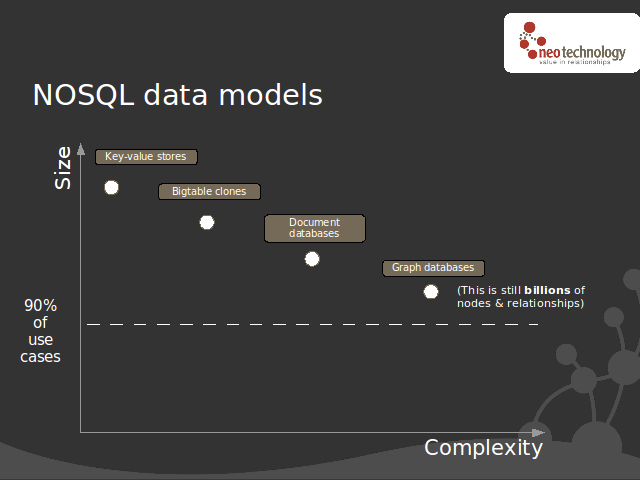
\includegraphics[width=16cm]{./figures/nosqldatamodels.png}
 % topologies802154.png: 722x407 pixel, 72dpi, 25.47x14.36 cm, bb=0 0 722 407
 \caption{Pozícia dátového modelu z pohľadu jeho škálovania podľa veľkosti a komplexnosti. Zdroj: Neo4J a NOSQL overview and the benefits of graph databases, Emil Eifrem, prezentacia.}
 \label{fig:scalling}
\end{figure}

Dátový model typu kľuč-hodnota a stĺpcovo orientovaný model (Bigtable clones) majú jednoduchú štruktúru, ktorá sa dá horizontálne škálovať. Nevýhodou tohoto prístupu je naopak to, že všetká práca s dátami a ich štruktúrou sa prenáša do vyšších vrstiev, o ktoré sa musí starať programátor. Naopak dokumentový a grafový model poskytuje bohatšiu štruktúru na prácu s dátami, ktorá spôsobuje komplikovanejšie škálovanie vhľadom na veľkosť dát. Podľa odhadov spoločnosti Neotechnology až 90\% aplikáci, v prípade že sa nejedná o projekty spoločností Google, Amazon atď., spadá do rozmedia kde sa veľkosť záznamov pohybuje rádovo v miliardách. Za zmienku stojí fakt, že aj napriek tomu, že tieto dátové modely sú si navzájom izomorfné, vhodnosť ich použitia závisí na konkrétnom príklade a požiadavkoch na aplikáciu. 

%one size fits all?
\subsection{Elastickosť}
Vďaka škálovaniu sa snažime o zýšenie kapacity celkového dátového úložiska. Elastickosť popisuje ako sa daný systém dokáže vysporiadať s pridaním nového uzlu.


\subsection{Konzistencia dát}
Poďla teórie CAP platí, že v prípade výskytu sieťových prerušení, ktoré sú súčasťou distribuovaného databázového systému nie je možné súčasne zaručiť vlasnosť konzistencie a dostupnosti. NoSQL systémy preto môžeme rozdeliť podľa tohoto modelu.

\begin{figure}[h]
 \centering
 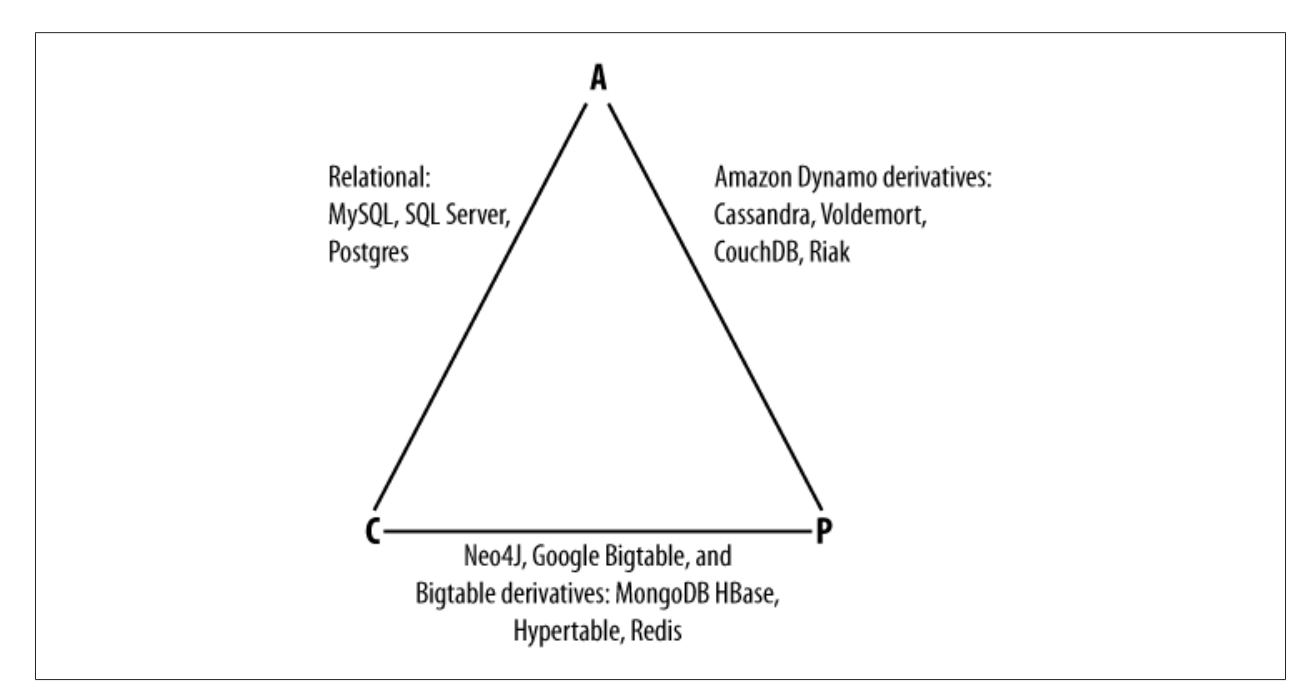
\includegraphics[width=16cm]{./figures/capDatabases.png}
 % topologies802154.png: 722x407 pixel, 72dpi, 25.47x14.36 cm, bb=0 0 722 407
 \caption{}
 \label{fig:scalling}
\end{figure}

Umiestnenie niektorých NoSQL datázových systémvo sa môže meniť podľa ich konfigurácie. 

Podpora replikácie, rozsekávania dát a zaradenie systému podľa modelu CAP určuje jeho dostupnosť.

\subsection{Perzistentné úložisko}
Typ perzistentného úložiska popisuje interný spôsob ukládania dát v databázovom systéme. NoSQL systémy môžu používať na ukládanie dát následujúce štruktúry: 
\begin{itemize}
 \item B-stromy
 \item distribuované hešové tabuľky
 \item Memtable / SSTable \footnote{Tieto štruktúry popíšeme v následujúcej sekcii}
 \item spojové zoznamy
 \item operačná pämeť, ktorej obsah je pravidelných intervaloch ukládaný na pevný disk
\end{itemize}
 
Podľa požiadavkov na našu aplikáciu sme čiastočne schopný odhadnúť pomocou, ktorej štruktúry by sme mohli dosiahnúť čo najefektívnejšiu výkonnosť.


%Snaha o globlálne výkonostné testy NoSQL systémov by viedla k porovnávaniu \uv{jabĺk s hruškami}.
%V následujúcej sekcii využijeme Yahoo! Cloud Serving Benchmark pre porovnanie nami vybraných kandidátov.

\section{Výber NoSQL systémov}
%http://themindstorms.blogspot.com/2009/05/quick-reference-to-alternative-data.html
%http://www.metabrew.com/article/anti-rdbms-a-list-of-distributed-key-value-stores

V predchádzajúcej sekcii sme tieto systémy rozdelili do štyroch hlavných kategórií podľa ich dátového modelu, ktorý je kľúčový pri výbere vhodného databázového systému podľa požiadavkov aplikácie. Popis a výkonnostné porovnanie NoSQL systémov, ktoré reprezentujú jednotlivé kategórie by boli nad rámec tejto práce. Paralelne s touto prácou vzniká diplomová práca, ktorá rieši podobný problém s využitím dokumentových databázových systémov  \ref{barina}, preto túto kategóriu vynecháme. 

Podľa analýzy požiadavkov na našu aplikáciu a štruktúry dát, ktoré budeme do databázového systému ukládať nie je vhodné použitie databázových systémov s grafovým modelom a modelom kľúč-hodnota. Systémy s grafovým modelom sú určené na diametrálne odlišnú úlohu problémov naopak v prípade, použita systémov kľúč-hodnota by bola práca na strane aplikácie zbytočne náročna. Našim požiadavkom najlepšie vyhovuje stĺpcovo orientovaný model, ktorý sme sa rozhodli použiť pre návrh našej aplikácie.

V tejto časti práce sa zameriame na stručný prehľad a vzájomné porovnanie systémov, ktoré poskytujú stĺpcovo orientovaný model. Medzi tieto voľne dostupné (open-source) systémy patria HBase, Cassandra a Hypertable. Aj napriek totožnému dátovemu modelu, majú tieto systémy odlišné vlasnosti. Následujúca tabuľka zobrazuje popis vlasností, na ktoré sme sa zamerali pri výbere víťaznej dvojice.



\begin{table}
    \begin{tabular}{|l|l|l|l|}
        \hline
        Vlastnosti/Databázový systém & Hbase & Cassandra & Hypertable \\  \hline
        Distribuovaný systém	& áno  & áno & áno \\ \hline 
        Dátový model		& Bigtable \footnote{lala} & Bigtable & Bigtable \\ \hline
        Dotazovací model	& ~  & ~ &  \\ \hline
	API 			& Thrift, REST  & Thrift, Avro & Thrift, C++ \\ \hline
        Perzistentné úložisko	& HDFS  & LSS\footnote{lokálny súborový systém} & HDFS, KFS, LSS \\ \hline
        SPOF \footnote{SPOF - uzol, ktorého nedostupnosť spôsobí nedostupnosť celého systému}	& áno  & nie & áno \\ \hline
	Pridanie uzlu do živého systému & áno  & áno & ~ \\ \hline
	Podpora viacerých datacentier & áno  & áno & áno \\ \hline
	Rozsekávanie dát 	& áno  & áno & áno \\ \hline
        Replikácia 		& pomocou HDFS  & áno & áno \\ \hline
	Elastickosť	        & áno  & áno & ~ \\ \hline
	Konzistencia 		& CP  & AP & ~ \\ \hline
	Programovací jazyk 	& Java  & Java & C++ \\ \hline
	MapReduce 		& áno  & áno & áno \\ \hline
	Komunita 		& +  & +  & - \\ \hline
    \end{tabular}
\end{table}


%porovnavane systemy sme vybrali podla citu , a taktiez spravyme benchmark od yahoo na 2 vybrane

Z porovania je vidieť, že systémy obsahuju množstvo spoločných vlastností. Pri výbere systémov sme zohľadnili aj ich praktické využitie spoločnostiami pôsobiacimi na trhu v produkčných podmienkách. Systém Cassandra je používaný spoločnosťou Facebook v aplikácii na súkromnú poštu. Medzi ďalšie požiadavky patrili podpora komunity, dokumentácia a vývojový cyklus týchto systémov. Z týchto systémov sme následne vybrali dva a to HBase a Cassandru. Dôvodom prečo sme zavrhli systém Hypertable je nepostačujúca dokumentácia, málo aktívna komunita a pomalý vývojový cyklus. V následujúcej sekcii popíšeme ich detaily.


\section{Cassandra}

Distribuovaný databázový systém Cassandra bol vytvorený pre interné účely spoločnosti Facebook v roku 2007. Cassandra slúžila na vyhľadávanie v súkromnej pošte, poskytovala úložisko pre indexy. Hlavnými požiadavkami na tento systém bolo zvládať miliardu zápisov denne, schopnosť škálovania podľa narástajúceho počtu použivateľov, beh na spotrebných počítačoch a podpora replikácie medzi geograficky oddelenými dátovými centrami. Ďalším požiadavkom bolo aby chyba žiadného uzlu nespôsobila celkovú nedostupnosť systému, teda systém bez SPOF. Cassandra je teda decentralizovaný systém, kde každý uzol je schopný vykonávať tie isté operácie. V roku 2008 bola zverejnená ako open-source projekt a je neustále vyvíjaná mnohými spoločnosťami a vývojármi. Tento systém využíva architektonické princípy distribuovaného databázového systému Dynamo vytvoreného spoločnosťou Amazon a zároveň ich kombinuje s dátovým modelom distribuovaného databázového systému BigTable vytvoreného spoločnosťou Google. V následujúcom texte popíšeme hlavne princípy tohoto systému.

\subsection{Dátový model}

Základný dátový model bol prebraný podľa Google Bigtable. Cassandra k nemu pridala ... 


Základnou jednotkou dátového modelu je stĺpec. Stĺpec je tvorený názvom, hodnotou a časovým odtlačkom, ktorý využíva Cassandra pri riešení konfliktov. Stĺpce sa zoskupujú do rodiny stĺpcov (Column family). Hodnoty zoskupených stĺpcov reprezentujú jeden záznam, ktorý identifikuje unikátny kľúč. Pomocou tohoto kľúča a názvu stĺpca sme schopný pristúpiť k hodnote ktorú reprezentuje. Pri vytváraní dátového modelu stačí vytvoriť rodinu stĺpcov a každý záznam, ktorý do nej vkládame môže obsahovať ľubovoľný počet stĺpcov. Tabuľkou je teda distribuovaná multidimenzionálna mapa, ktorá je indexovaná pomocou kľúčov. Operácie nad stĺpcami, ktoré identifikuje daný kľúč sú atomické. Ďalej platí, že vo v rámci rodiny stĺpcov sú stĺpce zoradené. Každá rodina stĺpcov je uložená v samostatnom súbore a je zoradená podľa kľúčov. Je preto vhodné do danej rodiny stĺpcov ukládať dáta, ku ktorým budeme pristupovať spoločne, čim sa vyhneme zbytočným diskovým operáciam.

Štruktúra super-stĺpec je špecialny typ stĺpca, ktorý je tvorenými obyčajnými stĺpcami. Stĺpec typu super má názov a jeho hodnota je tvorená zoznamom názvov obyčajných stĺpcov. Tento prístup pridáva ďalšiu úroveň v dátovej štruktúre. Tieto super stĺpce je možne združit do podobnej štruktúry a to super-rodiny stĺpcov. 

Uzol distribuovaného databázového systému obsahuje štruktúry pod názvom keyspace. U týchto štruktúr môžeme napríklad definovať faktor replikácie, môžeme sa na nich pozerať ako na databázu u relačných databázových systémov. Do štruktúry keyspace vkladáme rodiny stĺpcov, ktoré môžeme prirovnať k tabuľkám v relačných databázach. 


\subsection{ARchitektúra}








\section{Hadoop}

% podla porovnania vybereme 2 a tie dosledne popiseme 
% dovod preco sme vybrali column.familly - graf = komplexnost problemu narast data = a podla neho ze nepotrebujem key-value - zlozita praca so strukt. datami...  a popis 2 vybranych

\section{Hadoop vs. Cassandra}

%???Konflikty v distribuovanych DB ??? (vector clock)
%???? Výhody noSQL v porovnaní s modelovaním dát u relačných
% Štruktúra dát
% 
% Použitím relačných databáz podlieha návrh štruktúry dát predom známym návrhovým vzorom a normalizácií. Vyžaduje sa komplexná analýza vstupných dát a presná štrutúra dátového modelu tj. definovanie tabuliek, počet ich stĺpcov. Vývoj takýchto aplikácií sa prvotne zameriava na určenie štrukúry dát.
% 
% U množstva nových problémov ako napríklad grafy sociálnych sieti alebo vyhľadávače je komplikované predom určiť a popísať komplexne model dát, ktorý  sa môže časom  meniť, z dôvodu neustálej zmeny vstupných dát. V tomto prípade, nachádzame množstvo výhod u dátového modelu noSQL systémov, ktorý dokáže pracovať s neštrukturovanými alebo čiastočne štrukturovanými dátami.


\chapter{Analýza a návrh riešenia}







\chapter{ZMAZAT}
\section{Komponenty IEEE 802.15.4}
Zariadenia delíme na dva druhy a to zariadenie poskytujúce úplnú funkčnosť FFD (Full-function device) a redukované zariadenia RFD (Reduced-function device). Zariadenie FFD môže operovať v troch módoch, ktorými sú PAN (Personal area network) koordinátor, koordinátor, alebo koncové zriadenie. Zariadenie FFD ďalej dokáže komunikovať so zariadeniami typu RFD alebo FFD a zariadenie RFD je schopné komunikácie len so zariadením FFD. Výhodou RFD zariadení, je že neposielajú veľké objemy dát a teda na ich realizáciu je potrebná minimálna pamäťová kapacita. 
Samotná WPAN je tvorená dvoma alebo viacerými zariadeniami, ktoré komunikujú na tom istom fyzickom kanály.

\newpage 

\section{Sieťová topológia}

\begin{figure}[h]
 \centering
 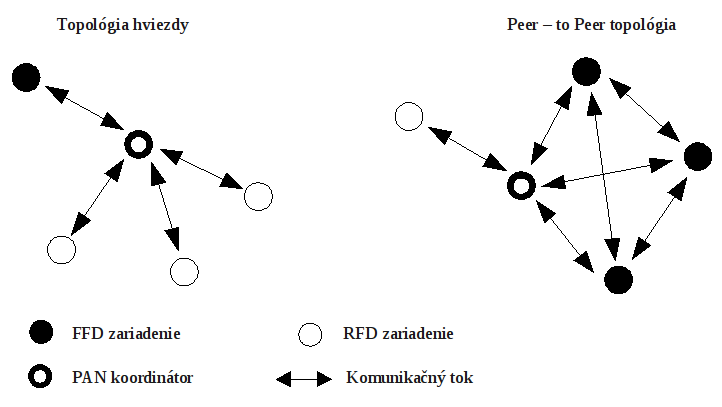
\includegraphics[width=12cm]{./figures/topologies802154.png}
 % topologies802154.png: 722x407 pixel, 72dpi, 25.47x14.36 cm, bb=0 0 722 407
 \caption{Topológie štandardu 802.15.4}
 \label{fig:80215topologies}
\end{figure}


\section{Architektúra}
Architektúra IEEE 802.15.4 viď. obrázok \ref{fig:802154layers} je tvorená pomocou vrstiev. Každá vrstva je zodpovedná za časť štandardu a poskytuje služby vyšším vrstvám. Vrstvy sú zavedené z dôvodu aby bol štandard ľahko popísateľný modelom ISO-OSI. 

LR-WPAN zariadenie je tvorené fyzickou vrstvou, ktorá zahŕňa rádiofrekvenčný vysielač, prijímač a mechanizmus potrebný na jeho obsluhu. Ďalšiu vrstvu tvorí linková vrstva, ktorá je zodpovedná za prístup všetkých prenosov ku komunikačnému kanálu. Jednotlivé vrstvy medzi sebou komunikujú pomocou prístupových bodov SAP (Service access point). Medzi vyššie vrstvy patrí sieťová vrstva a aplikačná vrstva, ktoré poskytujú zamýšľanú funkcionalitu zariadenia a patria do štandardu ZigBee. Architektúra LR-WPAN môže byť implementovaná u embeded zariadení a taktiež aj u zariadení vyžadujúcich pre svoj chod PC.



\begin{figure}[h]
 \centering
 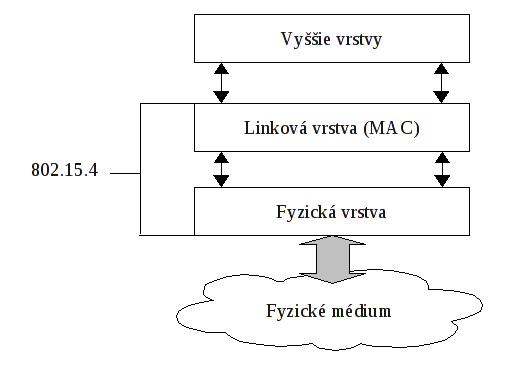
\includegraphics[width=10cm]{./figures/layers802154.png}
 % topologies802154.png: 722x407 pixel, 72dpi, 25.47x14.36 cm, bb=0 0 722 407
 \caption{Štruktúra štandardu 802.15.4}
 \label{fig:802154layers}
\end{figure}

\subsubsection{Typy rámcov}
Štruktúry rámcov boli navrhnuté aby zostala komplexnosť na minime, pri súčasnom zachovaní robustnosti pri posielaní dát na kanáli obsahujúcom šum.
Štandard definuje štyri druhy rámcov a to:
\begin{itemize}
\item beacon rámec
\item dátový rámec, ktorý sa používa pre prenos všetkých dát
\item potvrdzovací rámec, použitý k potvrdeniu úspešne prijatého rámca
\item MAC rámec, ktorý sa používa k spracovaniu všetkých servisných MAC prenosov
\end{itemize}

%TODO:
%?Režim spánku
%security page 24.



%  čím sa redukuje ich dopad na environmentálne prostredia a zaraďujeme ich do triedy zariadení, ktoré sa nazývajú Smart Energy. 
\section{Architektúra}
Architektúra štandardu ZigBee je tvorená viacerými blokmi, ktoré nazývame vrstvy. Každá z vrstiev vykonáva špecifickú množinu operácii, ktoré následne využívajú nadradené vrstvy. Ďalej sú použité dátové jednotky, ktoré sú zodpovedné za prenos dát a riadiace jednotky vykonávajúce všetky ostatné služby. Každá jednotka poskytuje svoje funkcie vyšším vrstvám pomocou rozhrania, ktoré sa nazýva SAP. Každé SAP rozhranie poskytuje množstvo servisných primitív, pomocou ktorých sa dosahuje požadovaná funkcionalita.
ZigBee aliancia stavia na základoch štandardu IEEE 802.15.4-2003, ktorý definuje dve vrstvy a to fyzickú vrstvu (PHY) a spojovú vrstvu (MAC), viď. predošlá kapitola. Nadstavbu týchto vrstiev tvorí sieťová vrstva (NWK) a framework aplikačnej vrstvy. Tento framework je ďalej tvorený vrstvou APS (Aplication support sub-layer) a vrstvou nazývanou ZDO (ZigBee device objects). Špecifické aplikácie daných výrobcov následne využívajú daný framework, vrstvy APS a objekty ZDO. Samotná architektúra je zobrazená na obrázku \ref{fig:ZigBeeLayers}

\begin{figure}[h]
 \centering
 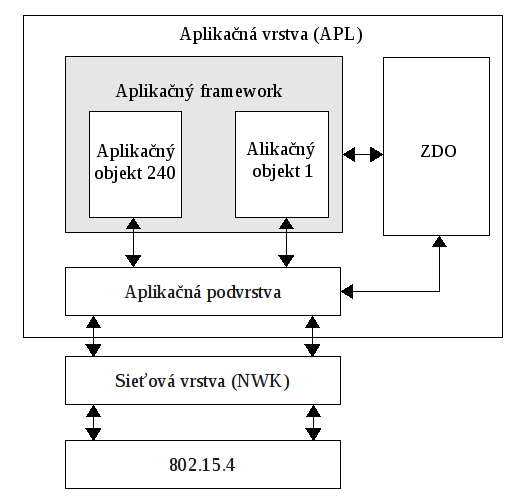
\includegraphics[width=10cm]{./figures/ZigBeeLayers.png}
 % topologies802154.png: 722x407 pixel, 72dpi, 25.47x14.36 cm, bb=0 0 722 407
 \caption{Štruktúra štandardu ZigBee}
 \label{fig:ZigBeeLayers}
\end{figure}

\section{Sieťové komponenty}
U sieti typu ZigBee rozoznávame nasledujúce tri druhy zariadení:
\begin{itemize}
\item ZigBee koordinátor, odpovedá PAN koordinátoru štandardu IEEE 802.15.4-2003
\item koncové zariadenie ZigBee, FFD alebo RFD zariadenie štandardu IEEE 802.15.4-2003, ktoré v ZigBee sieti nevystupuje ako ZigBee koordinátor alebo ZigBee smerovač
\item ZigBee smerovač, FFD zariadenie štandardu IEEE 802.15.4-2003, ktoré nemôže vystupovať v sieti ako ZigBee koordinátor, ale vystupuje ako koordinátor štandardu IEEE 802.15.4-2003, ktorý smeruje správy medzi zariadeniami a umožňuje asociáciu
\end{itemize}

\section{Sieťová topológia}
Sieťová vrstva štandardu ZigBee podporuje topológiu hviezda, ďalej stromovú a mesh (je to topológia používaná hlavne u bezdrôtových sieti, pri ktorej je každé sieťové zariadenie prepojené so všetkými ostatnými zariadeniami v danej sieti) topológiu.

\section{XBee Series 1}
Konkrétnu implementáciu predchádzajúcich štandardov tvoria moduly XBee/XBee PRO OEM od spoločnosti Digi, ktorá patrí do zoznamu certifikovaných výrobcov. V tejto práci som použil modul XBee Series 1, ktorý implementuje len štandard 802.15.4. Tento modul bol použitý pri meraniach v anténnej komore a jeho popisujúce parametre v samotnej simulácii. Linková vrstva modelu, ktorý som použil, pracovala s parametrami modulu TI CC1100, keď som chcel tieto parametre nahradiť, kontaktoval som spoločnosť Digi, ktorá mi však tieto parametre nebola schopná poskytnúť z dôvodu, že časť modulu, ktorá je zodpovedná za hodnoty týchto parametrov tvorí Ember 3.1 Stack, ktorý dodáva spoločnosť Ember. Spoločnosť Ember, však na moju žiadosť o sprístupnenie týchto parametrov (čas medzi prechodom z režimu spánku do režimu vysielania/prijímania, čas pri prechode zo stavu vysielania do stavu prijímania a opačne) vôbec nezareagovala.

\subsection{Technické parametre}
Modul popisujú následujúce parametre\cite{XBee}.

\begin{table}[htbp]
\begin{center}
\begin{tabular}{|c|c|}
\hline Dosah vnútri & 30m \\ 
\hline Dosah vonku & 90m \\ 
\hline Sila výstupného signálu & 1mW (0 dBm) \\
\hline Rýchlosť prenosu dát & 250 000 bps \\ 
\hline Rýchlosť sériového rozhrania & 1200 bps - 250 kbps \\ 
\hline Citlivosť pri príjme & -92 dBm \\
\hline 
\end{tabular} 
\end{center}
\caption{Špecifikácia výkonu a rýchlosti}
\label{tab:tab1}
\end{table}

\begin{table}[htbp]
\begin{center}
\begin{tabular}{|c|c|}
\hline Frekvenčné pásmo & ISM 2.4 GHz \\ 
\hline Rozmery & 2.438cm x 2.761cm \\ 
\hline Operačná teplota & -40 až 85C \\ 
\hline 
\end{tabular} 
\end{center}
\caption{Obecné parametre}
\label{tab:tab2}
\end{table}

\begin{table}[htbp]
\begin{center}
\begin{tabular}{|c|c|}
\hline Podporované sieťové technológie & Point-to-point, Point-to-multipoint, Peer-to-peer \\ 
\hline Počet kanálov & 16 \\ 
\hline Anténa & Whip \\
\hline Adresácia & PAN ID \\ 
\hline 
\end{tabular}
\end{center}
\caption{Sieťové parametre}
\label{tab:tab2}
\end{table}

\chapter{Teória antén}
Anténa je zariadenie, ktoré slúži na vysielanie a príjem rádiových signálov. Toto zariadenie konvertuje elektromagnetické vlny na elektrickú energiu a opačne. Podľa toho ako sú signály vysielané ich delíme na všesmerové (vysielanie vo všetkých smeroch) a smerové (vysielajú len v danom smere). Medzi chovaním sa vysielacej a prijímacej antény nepozorujeme žiadne rozdiely.

Následujúce parametre slúžia na popis základných vlastností antén:
\begin{itemize}
 \item smerovosť, určuje v akom smere sú elektromagnetické vlny vysielané. Je posudzovaná na základe vyžarovaných charakteristík, ktoré delíme na vertikálne a horizontálne. Meria sa pomocou parametrov zisk antény a vyžarovací uhol.
 \item vyžarovací uhol
 \item impedancia antény 
 \item zisk antény
 \item frekvenčná šírka prenášaného pásma
 \item polarizácia
 \item účinnosť
\end{itemize}

H rovina, je rovina v ktorej sa šíri vektor magnetického poľa a sleduje sa v nej ako sa mení intenzita elektrického poľa. Naopak v E rovine sa šíri vektor elektrického poľa a sleduje sa zmena intenzity magnetického poľa.

\subsection{Definícia pojmov}
Účinnosť je pomer vyžarovaného výkonu k výkonu, ktorý privádzame na vstup antény.
\linebreak 

\noindent Zisk určuje mieru smerovosti antény. Definujeme ho ako pomer vyžarovanej intenzity antény v danom smere k intenzite, ktorá je vyprodukovaná ideálnou anténou vyžarujúcou do všetkých smerov rovnomerne, bez strát a obe antény majú na vstupe rovnaký výkon. Zisk berie v úvahu okrem smerovosti aj účinnosť antény. Pre zisk ďalej platí, ak ma anténa pre daný smer väčší zisk ako je celkový zisk antény, tak v nejakom inom smere musí byť zasa zisk menší aby bola zachovaná celková energia. Tohoto faktu si je možno všimnúť u grafov popisujúcich zisk antén, ktoré boli vytvorené meraním v anténnej komore viď obrázok \ref{fig:xbeeWhipGain}.

%Relatívny zisk je pomer výkonového zisku pre daný smer k výkonovému zisku referenčnej antény vyžarujúcej v rovnakom smere. Vstupný výkon musí byť u oboch antén rovnaký. Referenčnou anténou je zvyčajne dipól alebo Horn anténa, u ktorých je hodnota vykonového zisku predom známa.

%Relative gain: The relative gain of a transmitting antenna in a given direction is defined as the ratio of the absolute gain of the antenna in the given direction to the absolute gain of a reference antenna in the same direction. The power input to the two antennas must be the same.

%smerovost = http://people.seas.harvard.edu/~jones/es151/prop_models/propagation.html#fsl

\subsection{Propagácia rádiového signálu}

Následujúci obrázok \ref{fig:RSP} zachytáva typický rádiový systém. Informácie vstupujú do vysielača. Informácie sú následne 
vysielané anténou, ktorá konvertuje rádiofrekvenčný signál na elektromagnetické vlny. Médium na prenos elektromagnetických vĺn je voľný priestor. Následne sú elektromagnetické vlny odchytené pomocou prijímacej antény, ktorá ich konvertuje spätne na rádiofrekvenčný signál. Ideálny stav je ak tento signál odpovedá signálu generovanému vysielačom. Originálna informácia, ktorá vstupovala do vysielača je následne demodulovaná na svoju pôvodnú formu.

\begin{figure}[h]
 \centering
 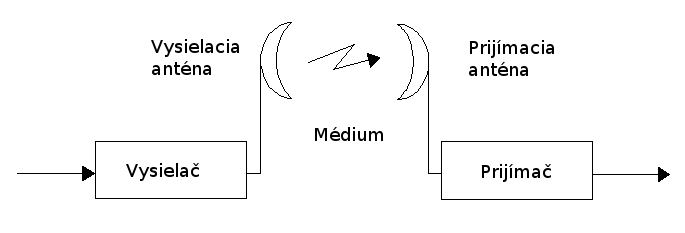
\includegraphics[width=10cm]{./figures/RSM.png}
 % topologies802154.png: 722x407 pixel, 72dpi, 25.47x14.36 cm, bb=0 0 722 407
 \caption{Model rádiového systému}
 \label{fig:RSP}
\end{figure}

\subsubsection{Pojmy}
\begin{itemize}
 \item dB - je skratka pre decibel. Je to matematické vyjadrenie používané na zobrazenie závislosti medzi dvoma hodnotami. 
 \item Rádiofrekvenčný výkon - je buď výkon vysielača alebo prijímača vyjadrený vo Wattoch. Taktiež môže byť vyjadrený v dBm. Vzťah medzi dBm a Wattmi je vyjadrený nasledovne $P_{dBm} = 10 * \log P_{mW}$
 \item Zoslabenie signálu modeluje nasledujúci obrázok \ref{fig:zoslab}. Kde Pin je vstupný výkon a Pout je hodnota výstupného výkonu.

 Zoslabenie je vyjadrené v dB podľa nasledujúceho vzťahu: $P_{dB} = 10 * \log(Pout / Pin)$. Napríklad predpokladajme, že dôjde k strate 1/3 vysielaného signálu (Pout/Pin = 2/3), potom hodnota zoslabenia v dB je 10 * log (2/3) = -4.05 dB
 
\item Citlivosť prijímača je minimálna hodnota výkonu radio frekvenčného signálu potrebná na vstupe prijímača, aby bol signál ďalej spracovaný. 

 \item Stratovosť je oslabenie výkonu radiofrekvenčneho signálu, ktorý je šírený v priestore. Je vyjadrená v dB a ďalej závisí na vzdialenosti medzi vysielacou a prijímacou anténou, na viditeľnosti medzi vysielacou a prijímacou anténou a na veľkosti antén.
\end{itemize}

\subsection{Typy antén}
\indent Izotropická anténa sa používa pre teoretické účely, vysielané vlny majú rovnaké parametre, ktoré popisujú anténu vo všetkých smeroch. Používa sa hlavne pri popisovaní a porovnávaní vlastností reálnych antén. 


\noindent Horn anténa sa používa v situácia, kde je potrebné dosiahnuť vysokého zisku, vlnová dĺžka je krátka, môže byť širokopásmová alebo úzko-pásmová, čo záleží na jej tvare. Taktiež dokáže pracovať s akoukoľvek frekvenciou. Keďže charakteristiky tejto antény sú známe a dobre matematicky popísané používa sa táto anténa ku kalibrácii iných systémov, tento fakt bol využitý aj počas meraní v anténnej komore. Hlavným parametrom, ktorý bol podstatný u meraní s touto anténou je jej zisk.


\noindent Whip anténa, je model antény, ktorý používajú ZigBee zariadenia, ktoré som simuloval. Anténa je poväčšine vertikálna a u ZigBee zariadení upevnená na doštičke plošného spoja. Je to anténa, ktorá vysiela horizontálne do všetkých smerov a hluché zóny sú vertikálne v bode upevnenia a ukončenia.

\subsection{Stratovosť voľného priestoru (Free-space path loss)}
%% http://www.radio-electronics.com/info/propagation/path-loss/free-space-formula-equation.php

Stratovosť signálu vo voľnom priestore sa používa k predikcii sily rádiového signálu. Napriek tomu, že nemodeluje dôveryhodne realitu obsahujúcu prekážky, odrazy atď, má veľký význam pre základné pochopenie šírenia sa signálu v reálnych podmienkach. Využíva sa taktiež pri tvorbe simulačných modelov a pri vývoji v oblasti bezdrôtových systémov.

Definujeme ju ako stratu sily signálu elektromagnetickej vlny, ktorá vzniká medzi dvoma priamo viditeľnými bodmi vo voľnom priestore, kde nie sú žiadne prekážky, odrazy a nedochádza k ohybu vĺn.

Formula pre výpočet stratovosti je nasledovná:
$$FSPL =  \left(\dfrac{4 \pi d}{\lambda}\right)^{2}  = \left(\dfrac{4 \pi d f}{c}\right)^{2},$$


kde:
\begin{itemize}
 \item $\lambda$ je vlnová dĺžka (m)
 \item f je frekvencia signálu (Hz)
 \item d je vzdialenosť od vysielača (m)
 \item c je rýchlosť svetla vo vákuu 2.99792458 * $10^{8}$ m/s
\end{itemize}

Daná formula vyjadrená v dB:

\begin{align*}
FSPL(dB) &= 10 \log_{10}\left(\dfrac{4 \pi df}{c} \right)^{2} \\
&= 20 \log_{10}\left(\dfrac{4 \pi df }{c} \right) \\
&= 20 \log_{10}(d) + 20 \log_{10}(f) + 20 \log_{10} \left(\dfrac{4 \pi}{c}\right)
\end{align*}


\subsection{Antény a simulácia}
Jednotlivé antény, na ktorých bolo vykonané meranie v anténne komore, boli popísané hodnotami výkonu (v dBm a W) v rozmedzí 0-360 stupňov pre každý stupeň. Z týchto hodnôt som pre každý stupeň spočítal hodnotu zisku. Samotný XML súbor, ktorý popisuje anténu a je použitý k simulácii potom obsahuje hodnoty ziskov po 10 stupňov, ktoré som spočítal ako priemer z hodnôt z meraní, čo samozrejme spôsobí ďalšiu odchýlku od reality. \\

%popis pocitania?


\begin{figure}[htbp]
 \centering
 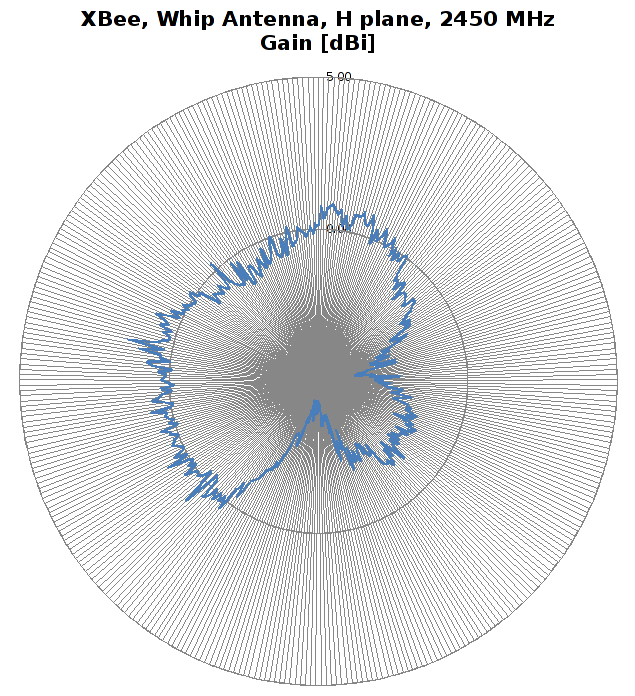
\includegraphics[width=9cm]{./figures/xbeeWhipGain.png}
 % topologies802154.png: 722x407 pixel, 72dpi, 25.47x14.36 cm, bb=0 0 722 407
 \caption{Charakteristika zisku antény Whip}
 \label{fig:xbeeWhipGain}
\end{figure}


\begin{figure}[htbp]
 \centering
 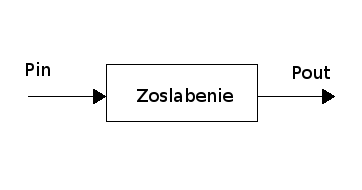
\includegraphics[width=8cm]{./figures/zoslabenie.png}
 % topologies802154.png: 722x407 pixel, 72dpi, 25.47x14.36 cm, bb=0 0 722 407
 \caption{Model zoslabenia signálu}
 \label{fig:zoslab}
\end{figure}


%%TODO:
%% 2 obrázky



%%%
\begin{verbatim}
inicializácia - vybudovanie modelu a vloženie prvých udalosti do FES

while(FES nie je prázdna a simulácia neskončila) 
{
	vyber prvú udalosť z FES
	t:= sprav časovú značku tejto udalosti
	spracuj udalosť
	(spracovanie udalosti môže pridať novú udalosť alebo zmazať existujúcu z FES)
}

ukončenie simulácie (zápis výsledkov, atď.)
\end{verbatim}
%%%




%*****************************************************************************
\chapter{Analýza a návrh riešenia}
%Analýza a návrh implementace (včetně diskuse různých alternativ a volby implementačního prostředí).


\subsubsection{Výkonová závislosť}
%% http://en.wikipedia.org/wiki/Link_budget

Následujúci obrázok \ref{fig:FSPL} zobrazuje vysielač (T), u ktorého vystupuje dvojica výkonov $P_{1}$, $P_{2}$ a hodnota zisku pre daný smer $G_{T}(\alpha_{T})$, ďalej u prijímača (R) vystupujú výkony $P_{3}$, $P_{4}$ a zisk v danom smere $G_{R}(\alpha_{R})$. V simulácii bude zohrávať hlavnú úlohu hodnota výkonu $P_{4}$, hodnota výkonu $P_{1}$ je pred vyslaním rámcu známa, je to hodnota špecifikovaná výrobcom zariadenia. V následujúcej časti odvodím vzťah pomocou, ktorého určím hodnotu výkonu $P_{4}$, na základe ktorej sa prijímač rozhodne či sa naozaj jedná o prijímané dáta alebo sa vysielaný signál zoslabil na takú úroveň, kedy bude považovaný za šum na kanály.

Nasleduje formula pre výpočet hodnoty výkonu $P_{4}$, pomocou FSPL:

\[
\left[\frac{P_{3}}{P_{2}}\right]_{W} =\left(\frac{\lambda}{4\pi}\right)^{2}\frac{1}{d^{\alpha}}
\]

\begin{align*}
\left[\frac{P_{3}}{P_{2}}\right]_{dB} &= 10\log_{10}\left(\frac{\lambda}{4\pi}\right)^{2}\frac{1}{d^{\alpha}} \\
&= 10\log_{10}\left(\frac{c}{4\pi f}\right)^{2}\frac{1}{d^{\alpha}} \\
&= 20\log_{10}\left(\frac{c}{4\pi f}\right)-10\alpha\log_{10}d \\
&= -40.2251-10\alpha\log_{10}d, 
\end{align*}

kde:
\begin{itemize}
 \item $\lambda$ je vlnová dĺžka (m), $\lambda = \frac{c}{f}$
 \item f je frekvencia signálu (Hz), pre použité zariadenia XBee f = 2450 Mhz
 \item d je vzdialenosť od vysielača (m)
 \item c je rýchlosť svetla vo vákuu 2.99792458 * $10^{8}$ m/s
 \item $\alpha$ je koeficient útlmu prostredia (pre vzduch $\alpha = 2$)
\end{itemize}

Zavediem nasledujúce označenie:
$$L = -40.2251 - 10\alpha\log_{10}d$$

Ďalej platí:
\[
P_{2} = P_{1} + G_{T}(\alpha_{T}) \]
\[
P_{3} = P_{2} + L \]
\[
P_{4} = P_{3} + G_{R}(\alpha_{R}), \]

z čoho následne vyplýva následujúca rovnosť:
$$
P_{4} = P_{1} + G_{T}(\alpha_{T}) + G_{R}(\alpha_{R}) + L + K,
$$

kde:
\begin{itemize}
 \item $P_{1}$ - výkon privedený do antény vysielača (dBm)
 \item $P_{2}$ - výkon vysielaný vysielacou anténou (dBm)
 \item $P_{3}$ - hodnota výkonu prijatého prijímacou anténou (dBm)
 \item $P_{4}$ - výkon vystupujúci z káblu prijímacej antény a vstupujúci do prijímača (dBm)
 \item $G_{T}(\alpha_{T})$ - zisk vysielacej antény v danom smere (dBi)
 \item $G_{R}(\alpha_{R})$ - zisk prijímacej antény v danom smere (dBi)
 \item K - konštanta, ktorá spôsobuje ďalšie straty existujúce v reálnom prostredí (odrazy vo vodičoch, konektoroch, atď.)
\end{itemize}

Taktiež zároveň platí:
$$
P_{4}^{'} < P_{4}^{''},
$$

kde:
\begin{itemize}
 \item $P_{4}^{'}$ - hodnota výkonu v reálnom prostredí (W) 
 \item $P_{4}^{''}$ - spočítaná hodnota výkonu $P_{4}$ (W)
\end{itemize}

$$
\left[P_{3}\right]_{W} < \left[P_{2}\right]_{W} => \left[\frac{P_{3}}{P_{2}}\right]_{dB} < 0.
$$

Daný vzťah uvažuje straty, ktoré vznikajú na konektoroch antén, prepojovacím káblom medzi anténou a zariadením, vlastným odporom vodiča antény a iné. v podobe konštanty K.

%kedze model dokonalo modelujuci realne prostredie je zlozity... zameriame sa len na jeho cast ktorou v ktorej popiseme realne sa spravanie anten. anteny by boli uvazovane ze do vsetkych smeroch maju rovnaky zisk co je omyl... doplnenie modelu MiXmiX nasim realnym popisom anten bude o to realistickejsie.
%teoria k tomu ako sa riesi simulacia realneho prostredia 
%Rádio frekvenčné signály sa prenášajú veľmi rýchlo, no počas ich prenosu môže dochádzať k ich strate poprípade odrazom.

\begin{figure}[htbp]
 \centering
 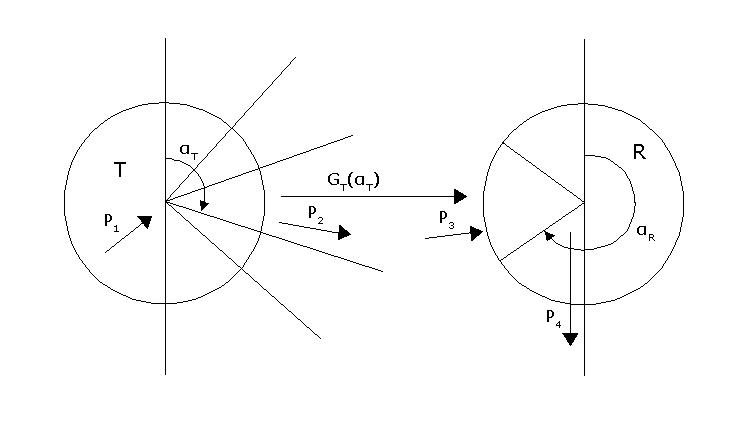
\includegraphics[width=10cm]{./figures/FSPL.png}
 % topologies802154.png: 722x407 pixel, 72dpi, 25.47x14.36 cm, bb=0 0 722 407
 \caption{Popis výkonov a zisku u antén pre vysielač a prijímač}
 \label{fig:FSPL}
\end{figure}


\subsection{Štruktúra MF}
V tejto časti sa zameriam na detailný popis funkcie modulov a ich následnú implementáciu. Obrázok \ref{fig:Host} zachytáva štruktúru stanice, ktorú popisujeme pomocou jazyka NED. Na základe konvencie musí názov súboru vo svojom názve obsahovať reťazec \uv{host}. Ako môžeme vidieť daná stanica sa skladá z jednotlivých podmodulov a to aplikačná vrstva, sieťová vrstva a vrstva NIC, ktoré navzájom komunikujú. Stanica taktiež obsahuje modul \textit{Mobility}, ktorý zabezpečuje pohyb a geografickú pozíciu uzlu. 

Podmoduly modulu stanica majú spoločného predka, ktorým je trieda \textit{BasicModule}. Táto trieda je ďalej potomkom triedy \textit{cSimpleModule}, ktorá je súčasťou Omnetu. Trieda \textit{BasicModule}, obsahuje dvojfázovú inicializáciu, ktorá je vhodná aj v prípade použitia modulu \textit{Blackbox} \footnote{Je to modul umožňujúci medzivrstvovú komunikáciu, bez nutnosti zasielania správ}, ktorý v tomto texte nebudem popisovať. Medzi ďalšie vlastnosti patrí napríklad metóda \textit{logName}, ktorá vracia názov NED modulu, čo je možné využiť pri ladení za pomoci makra EV, ktoré slúži pre výpis ladiacich správ. 

Samotná komunikácia medzi jednotlivými podmodulmi modulu stanice je zabezpečená pomocou metód:
\begin{itemize}
 \item \textit{handleUpperMsg} - táto metóda je volaná zakaždým, keď modul obdrží správu z vyššej vrstvy, následne ju spracuje a predá nižšej vrstve
 \item \textit{handleLowerMsg} - metóda je volaná po príchode správy z nižšej vrstvy, správu ďalej spracuje a predá nadradenej vrstve
\end{itemize}

Ďalej sú k dispozícii pomocné metódy slúžiace k enkapsulácii a dekapsulácii správy predávanej medzi vrstvami (\textit{encapsMsg, decapsMsg}) a metódy na opozdenie správy pri jej vysielaní na kanál.

Keďže model poskytuje enkapsuláciu a dekapsuláciu správ, z toho vyplýva, že pre každú vrstvu definujeme osobitný typ správy, ktorej štruktúra je popísaná pomocou súboru s príponou .msg. K dispozícii sú napríklad správy typu \textit{AirFrame} (správa pre komunikáciu na fyzickej vrstve), \textit{MacPkt} (správa pre komunikáciu na linkovej vrstve), \textit{NtwPkt} (správa pre sieťovú vrstvu) a \textit{ApplPkt} (správa pre vrstvu aplikačnú). Všetky typy správ sú rozšíriteľné, resp. si pomocou nich môžeme odvodiť vlastný typ správy. Pre potreby mojej simulácie bola najdôležitejšia správa typu \textit{AirFrameRadioAccNoise3}, zdedená z triedy \textit{AirFrame}, ktorej štruktúra obsahuje následujúce položky

\begin{itemize}
 \item pSend - výkon, ktorým bol rámec odoslaný
 \item channelId - kanál, na ktorý bola správa zaslaná
 \item duration - čas, ktorý bol spotrebovaný na zaslanie rámcu (v sekundách)
 \item hostMode - štruktúra popisujúca pozíciu stanice, jej rýchlosť, smer pohybu, čas kedy sa pohyb začal
 \item SnrControlInfo - trieda, ktorá obsahuje pomocné informácie SNR (Signal to noise ratio), ktoré sa predávajú modulu \textit{Decider}
\end{itemize}

%snr infor z MSG decideru a z nich spocitame bit errors

Danú správu som ďalej rozšíril o parameter moduleId, ktorý obsahuje globálny identifikátor modulu, z ktorého bola správa odoslaná.

\begin{figure}[h]
 \centering
 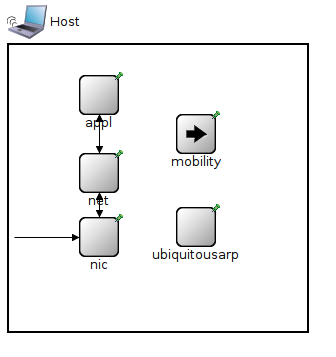
\includegraphics[width=6cm]{./figures/host.png}
 % topologies802154.png: 722x407 pixel, 72dpi, 25.47x14.36 cm, bb=0 0 722 407
 \caption{Štruktúra stanice v OMNeT++}
 \label{fig:Host}
\end{figure}

\subsubsection{Štruktúra modulu NIC}

%% finut tie pojmy  ,, mac vrstva == spojova ?
NIC (Network card interface) je časť sieťového adaptéru zodpovedná za fyzický prístup k médiu a adresácii na úrovni MAC vrstvy, popisuje ju fyzická a linková vrstva ISO-OSI modelu. Štruktúra tohoto modulu je znázornená na obrázku \ref{fig:Nic}. V mojom prípade je teda fyzická vrstva tvorená modulom \textit{snrEval}, \textit{decider} a vrstvu MAC tvorí modul \textit{mac}. Vzájomná úzka kooperácia medzi týmito vrstvami je dôvodom prečo sú zapuzdrené v jednom module. Všetky submoduly modulu NIC, sú zdedené z triedy \textit{ChannelAcces}, ktorá je ďalej odvodená z triedy \textit{BasicModule}. Táto trieda poskytuje funkcionalitu umožňujúcu komunikáciu jednotlivých staníc, ktoré sú vo vzájomnom dosahu. Na úrovni fyzickej vrstvy ma hlavne zaujíma modelovanie oslabenia signálu a výpočet chybovosti na kanále. Tým, že je fyzická vrstva tvorená osobitne modulom \textit{snrEval}, som schopný modelovať výpočet stratovosti na kanále pomocou rôznych metód a na základe výsledku sa v module \textit{decider} rozhodnem pomocou akého kritéria tieto dáta vyhodnotím. Napríklad modul \textit{decider} bude rozhodovať o tom či dané dáta príjme na základe porovnania hodnoty SNR, spočítanej z modulu \textit{snrEval}, s definovanou hraničnou hodnotou, alebo sa môže rozhodovať na základe počítania pomocou formúl pre výpočet chybovosti na kanále (napr. BER). Vďaka tomu môžem tieto moduly navzájom rôzne kombinovať. V následujúcej časti detailnejšie priblížim štruktúru modulov \textit{snrEval} a \textit{decider}. \\


\noindent\textbf{Modul snrEval}

Tento modul zabezpečuje príjem a vysielanie dát na kanál. Ďalej vytvára správy typu \textit{AirFrame} z \textit{MacFramu} a opačne, počas toho ako odpočúva kanál zároveň mení stavy rádia, ktoré sú reprezentované stavovým automatom a taktiež zabezpečuje simuláciu oneskorenia vo vysielaní alebo príjme pomocou pomocných funkcií (\textit{bufferMsg, unbuefferMsg}). V mojom modele ma zaujímala jedna z jeho ďalších vlastností a to ukladanie a spracúvanie SNR hodnôt pri prijímaní rámcov. Rámec fyzickej vrstvy (\textit{AirFrame}) obsahuje pomocnú štruktúru \textit{SnrList}, ktorú reprezentuje štruktúra \textit{List} programovacieho jazyka C++ a záznam tejto štruktúry obsahuje dve položky a to časovú značku prijatia rámcu a k nej odpovedajúcu hodnotu SNR. V mojom prípade je hodnota SNR spočítaná na základe vzťahu [hodnota výkonu vstupujúca do prijímača ($P_{4}$) / hodnota šumu na kanále], kde hodnotu $P_{4}$ počítam za využitia modifikovanej formule FSPL. Túto hodnotu následne predávam do modulu \textit{Decider}, kde je ďalej spracovaná.

Práca modulu snrEval je znázornená vývojovým diagramom na obrázku \ref{fig:snrEval}. Keď sa nachádza modul v stave SYNC prijíma správu. Pred jej prijatím sa najskôr vykoná kontrola, či nedošlo k poškodeniu SFD (Start frame delimiter), následne sa spracuje zvyšok správy a spočíta sa hodnota SNR. V prípade, že sa modul nenachádza v stave SYNC a obdrží ďalšiu správu je tato správa považovaná za šum, hodnota šumu sa zvýši o hodnotu výkonu, ktorým bola táto správa prijatá a spočíta sa nová hodnota SNR, ku ktorej je pripojená časová značka. Detailnejšie sa budem zaoberať modelom kolízie v následujúcej kapitole.

%% rcdPower / noiseLevel

V tomto module je metóda \textit{handleLowerMsg} rozdelená na dve časti a to:
\begin{itemize}
 \item \textit{handleLowerMsgStart} - volá sa hneď po prijatí správy, volá metódy na výpočet hodnoty prijatého výkonu ($P_4$) a následne predáva spracovanie ďalším metódam na základe stavu rádia
 \item \textit{handleLowerMsgEnd} - slúži na samotné odoslanie správy vyššej vrstve a zároveň pripája \textit{SnrList} ako parameter.
\end{itemize}


\noindent\textbf{Modul decider}
 
Modul spracúva len správy, ktoré prichádzajú z kanálu cez modul \textit{SnrEval}. Správy z vyšších vrstiev, ktoré sa posielajú na kanál neprechádzajú týmto modulom a to z dôvodu, že tento modul len rozhoduje, či sa daná správa zahodí alebo prepošle vyššej vrstve. Rozhodovanie je založené na základe výpočtov ako napríklad chybovosť bitov alebo sa rozhoduje či sa má správa zahodiť na základe vysokej hodnoty šumu na kanále porovnaním s hraničnou hodnotou. Tieto vlastnosti však sledujem len u správ prichádzajúcich z kanálu. \textit{Decider} teda slúži na výpočet chybných bitov (BER) v správe, čo počíta pomocou hodnôt uložených v štruktúre \textit{SnrList}. Ďalej je v ňom možné implementovať rôzne opravné kódy. V simulácii je použitý vzorec na výpočet chybných bitov (BER) pre moduláciu MSK. 
$$BER = 0.5 * exp(-0.5 * SNR)$$


Modul \textit{mac} ďalej poskytuje funkcionalitu metódy na riadenie prístupu k médiu CSMA. Modul \textit{radio} je centrálne zdieľaný a moduly ako \textit{snrEval} alebo \textit{mac} prepínajú jeho stavy (napr. RX, TX) podľa potreby. Posledným modulom, je modul \textit{antenna} ktorý popisuje parametre antény a je využívaný modulom \textit{snrEval}.

%\subsubsection{Mobiná architektúra a správa komunikačného kanálu} 

\begin{figure}[h]
 \centering
 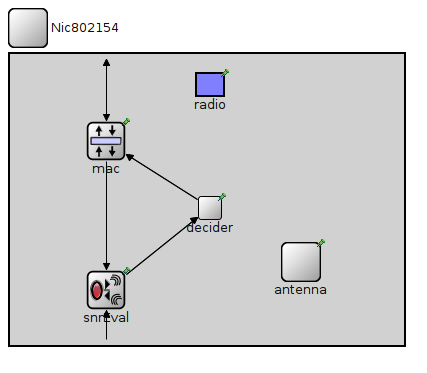
\includegraphics[width=8cm]{./figures/nic.png}
 % topologies802154.png: 722x407 pixel, 72dpi, 25.47x14.36 cm, bb=0 0 722 407
 \caption{Štruktúra NIC v OMNeT++}
 \label{fig:Nic}
\end{figure}

\begin{figure}[h]
 \centering
 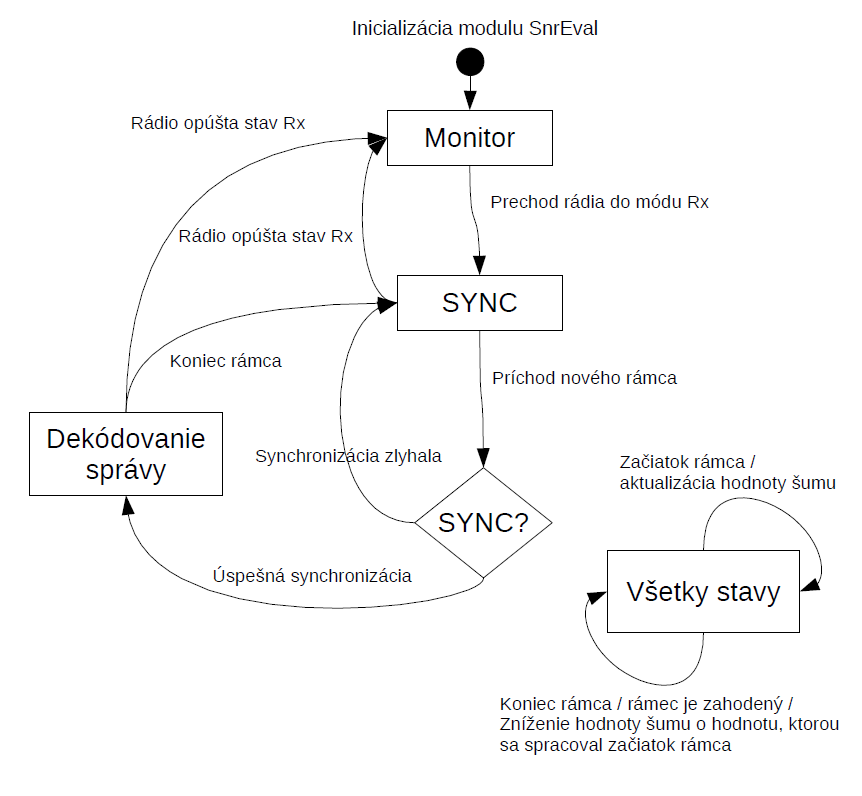
\includegraphics[width=13cm]{./figures/snrEval.png}
 % topologies802154.png: 722x407 pixel, 72dpi, 25.47x14.36 cm, bb=0 0 722 407
 \caption{Prechody medzi stavmi v module snrEval}
 \label{fig:snrEval}
\end{figure}

%*****************************************************************************
\chapter{Realizácia}

Pre potrebu simulácie som teda ako prvý vytvoril modul \textit{Antenna}, ktorý popisuje anténu ZigBee zariadení následujúcimi parametrami:
\begin{itemize}
 \item zisk - ideálny zisk antény, ktorý nájdeme v popise antény (dBi)
 \item impedancia ($\Omega$)
 \item config - odkazuje na xml súbor popisujúci zisk antény (*.xml)
\end{itemize}

Modul sa snaží byť čo najobecnejší pre prípadne využitie aj v iných modeloch a pridal som ho medzi ostatné moduly MF. Z predošlých parametrov je najdôležitejší parameter \textit{config}. Pomocou tohoto parametru sa odkazujem na súbor, ktorým popisujem zisk antény pre daný uhol, v ktorom anténa prijíma alebo vysiela. Hodnoty tohoto súboru sú z meraní, ktoré boli vykonané v anténnej komore. Nasledujúce riadky zachytávajú príklad popisu konkrétnej antény. 

\begin{verbatim}
<?xml version="1.0" encoding="UTF-8"?>
<!DOCTYPE antenna SYSTEM "Antenna.dtd">
<antenna>
        <angle min="0" max="0" gain="0.3" />
        <angle min="0" max="30" gain="0.4" />
        <angle min="30" max="360" gain="0.9" />
<antenna>
\end{verbatim}

Jednotlivé záznamy v elementoch <angle ...>, reprezentujú hodnotu zisku pre uhol z intervalu (min, max>. Jednotlivé intervaly musia byť zoradené vzostupne, bez prekrývania sa. V prípade, že je rámec odoslaný pod uhlom ktorý, sa v popisnom xml súbore nenachádza, je použitá  hodnota ideálneho zisku, ktorá je zapísaná v .ned súbore popisujúcom štruktúru modulu antény. Táto hodnota môže byť prepísaná v konfiguračnom súbore danej simulácie omnetpp.ini pomocou nasledujúceho zápisu: 
sim.host[*].nic.antenna.gain = 2.1dBi

Parametru \textit{config}, ktorý odkazuje na xml súbor je potrebné priradiť xml súbor aj v prípade ak chcem v simulácii použiť len hodnotu teoretického zisku antény. V aktuálnej verzii Omnetu nie je možné priradiť tomuto parametru napríklad hodnotu \uv{false} a zabezpečiť týmto neodkazovanie sa na xml súbor. Túto funkcionalitu som ďalej do Omnetu neimplementoval, pretože po konzultácii s autorom Omnetu, som sa dozvedel, že táto možnosť pribudne v jeho novej verzii. Tento prípad riešim tak, že parametru config priradím xml súbor obsahujúci samotný koreňový element <root />, ktorý vyhodnotím pri samotnom spracúvaní xml súboru.

Samotný xml súbor popisujúci konkrétny model antény priradím danej stanici následovne: sim.host[*].nic.antenna.config = xmldoc(\uv{antenna1.xml})

%validuje???
Po spustení simulácie sa v inicializačnej časti modulu validuje daný xml súbor pomocou súboru Antenna.dtd, ďalej sa načíta do pamäti, z dôvodu, že simulátor poskytuje len DOM parsér a sprístupním si odkaz na jeho prvý element <angle ...>. Modul ďalej obsahuje metódu \textit{findGainValue}, ktorá v danom xml súbore vyhľadá hodnotu zisku pre daný uhol. Z dôvodu optimalizácie som pre vyhľadávanie v štruktúre xml súboru použil binárne vyhľadávanie.

Ďalej som do modulu \textit{SnrEvalRadioAccNoise3} implementoval výpočet modifikovanej formule FSPL. Samotný priestor, takzvaný playground, v ktorom sa odohráva simulácia som rozdelil na štyri kvadranty, vďaka čomu dokážem veľmi efektívne počítať uhol, pod ktorým bol rámec vyslaný z vysielacej stanice a uhol, pod ktorým bol rámec prijatý na prijímacej stanici. Tieto uhly sú prepočítané na strane príjemcu, z ich hodnôt zistím pomocou modulu antény, konkrétne hodnoty daných ziskov $G_{T}(\alpha_{T})$ a $G_{R}(\alpha_{R})$. Hodnotu zisku $G_{R}(\alpha_{R})$ určím priamo pomocou metódy \textit{faindGainValue} modulu \textit{antenna}, ktorý obsahuje prijímač. Prijatý rámec obsahuje hodnotu jedinečného identifikátoru modulu (moduleId), z ktorého bol vyslaný. Pomocou neho sprístupním odkaz na modul vysielača a taktiež zavolám jeho metódu \textit{findGainValue}, ktorá mi vráti hodnotu zisku $G_{T}(\alpha_{T})$. Následne môžem spočítať hodnotu výkonu $P_4$, z tejto hodnoty sa ďalej spočíta hodnota SNR pomocou vzťahu SNR = $P_4$/[hodnota šumu prostredia], kde hodnota šumu prostredia je rovná -100dBm. SNR sa ďalej pripojí ako kontrolná informácia k rámcu a odošle o úroveň vyššie vrstve \textit{decider}. Táto vrstva následne spočíta hodnotu BER pre daný rámec a v prípade, že nedošlo k poškodeniu rámca je tento rámec predaný opäť vyššej vrstve a to vrstve MAC.

Pre potreby vyhodnocovania modelov, som ďalej upravil modul \textit{ChannelControl}, kde bol pridaný parameter ratio, pomocou, ktorého je prepočítavaná vzdialenosť v modeli na reálnu vzdialenosť.

Počas implementácie a ladenia modelu som objavil v produkčnom kóde MF, dve chyby, konkrétne pri výpočte hodnoty BER v module \textit{decider}, druhá chyba bola v module \textit{snrEval}. Po upozornení autora boli obe chyby opravené.

% Popis vrstvy APPL layer
%V mojom prípade som v module snrEval zmenil a pridal to a to
%??? a v module decider som pouzit - pridal - zmenil to a to.

%kolizia.png

\subsection{Model kolízie}
Pri komunikácii ZigBee zariadení v reálnom prostredí môže dochádzať k ich vzájomnému rušeniu. Takáto situácia môže nastať napríklad v prípade, že nastane kolízia v mechanizme, ktorý riadi prístup k médiu (CSMA-CA) alebo ak máme dve siete, kde prijímač z prvej siete príme súčasne v jednom okamihu počas svojho stavu Rx, dva rámce. Súčasné prijatie dvoch rámcov na anténe zanesie do komunikácie šum (čo je vlastne prídavný signál), ktorý môže ďalej spôsobiť chybovosť (BER). Keďže, som chcel modelovať aj situácie, u ktorých by dochádzalo k rušeniu, musel som pre tieto potreby model čiastočne modifikovať. Daný model neposkytuje vrstvy štandardu ZigBee preto nie je možné modelovať dve nezávislé siete. Danú kolíziu som preto vytvoril pomocou modifikácie MAC vrstvy, čím som dosiahol, že dané zariadenie sa chovalo ako generátor šumu, tj. periodicky vysiela rámce, s tým, že dochádza ku kolízii a prijímač príjme viacero rámcov súčasne.

V simulácii je používaný diskrétny simulátor, počas simulačného času prebiehajú udalosti. Model súčasného prijatia viacerých rámcov vyzerá tak, že v čase keď prijímač príjme rámce simulačný čas sa zastaví a samotné prijatie rámcov považujeme za udalosti v rovnakom simulačnom čase. Procesorový čas však neustále beží a teda program obsluhujúci súčasne prijatie viacerých rámcov príjme tieto rámce v skutočnosti s určitým časovým odstupom, čo je v simulácii reprezentované pomocou udalosti. Najprv je prijatý prvý rámec, je spracovaná jeho obsluha, následne sa spracuje druhý rámec atď. Tomuto popisu odpovedá nasledujúci obrázok \ref{fig:kolizia}, ktorý zachytáva situáciu pri ktorej došlo ku kolízii v modifikovanej vrstve MAC (modul \textit{mac}).

\subsubsection{Popis kolízie}
Obrázok \ref{fig:kolizia} je výstup z nástroja Sequence chart a detailný popis jednotlivých udalosti je možné analyzovať pomocou nástroja Event log. Oba tieto nástroje sú vhodné pre analýzu simulácie poprípade jej ladenie a pribudli vo verzii OMNeT++ 4.0. V mojom modely \ref{fig:modelKolizie} som simuloval vznik kolízie na module host[0], ktorý periodicky prijímal rámce z modulu host[1]. Modul host[2] som použil ako generátor rámcov, ktoré budú spôsobovať kolízie. Na obrázku reprezentuje sivý úsek zastavenie simulačného času. Modul host[0] prijal v rovnaký čas dva rámce, prvý od modulu host[1], čomu odpovedá číslo udalosti 41, druhý od modulu host[2] s číslom udalosti 43. Oba tieto rámce boli prijaté modulom \textit{snrEval}. Na základe predchádzajúceho popisu modulu \textit{snrEval}, prebehne následujúca obsluha:
\begin{enumerate}
 \item rámec z udalosti 41, vstupuje do modulu \textit{snrEval}, ktorý sa sa prepne do stavu SYNC, keďže sa jedná o nový rámec, je spočítaná hodnota SNR1, nasleduje prepnutie do stavu Dekódovanie správy \\ \\
 SNR1 = (výkon, ktorým bol rámec prijatý / šum)
 \item následne je prijatý rámec z udalosti 43, tento rámec bude spracúvaný ako šum, spočíta sa nová hodnota SNR2, rámec sa následne zahodí \\ \\
 SNR2 = (hodnota výkonu, ktorým bol prijatý rámec z udalosti 41) / (šum + prijatý výkon rámca z udalosti 43)
 \item ukončí sa spracovanie rámca z udalosti 41, hodnoty SNR1 a SNR2 sa pripoja ako kontrolné informácie k správe, ktorá sa následne prepošle modulu \textit{decider}
 \item \textit{decider} na základe hodnôt SNR1, SNR2 spočíta BER a podľa jeho hodnoty sa rozhodne či sa rámec zahodí (tj. rámec obsahuje chybné bity) alebo pošle modulu \textit{mac}
\end{enumerate}

Čím je nižšia hodnota SNR, tým je vyššia pravdepodobnosť, že prijatý rámec bude obsahovať chyby. Tento fakt vychádza zo Shannonovej vety, danej nasledujúcou formulou, ktorá udáva max. teoretický limit prenosovej rýchlosti C kanálu s pásmom o šírke W a odstupom signálu od šumu (SNR).

$$ C = W * \log_{2} (1 + SNR) [b/s, Hz] $$

V prípade, že sa hodnota SNR blíži k nule, prenosová rýchlosť kanálu sa taktiež blíži k nule, z čoho vyplýva, že dochádza k veľkej strate prenášaných dát, čo zapríčiní veľkú chybovosť na prenášaných dátach. \\

\begin{figure}[h]
 \centering
 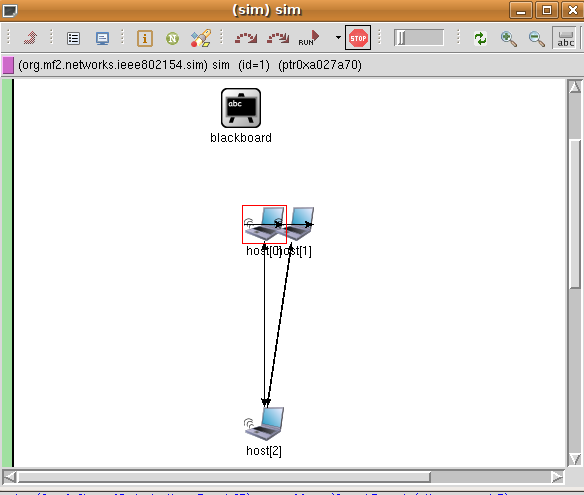
\includegraphics[width=10cm]{./figures/modelKolizie.png}
 % topologies802154.png: 722x407 pixel, 72dpi, 25.47x14.36 cm, bb=0 0 722 407
 \caption{Model kolízie}
 \label{fig:modelKolizie}
\end{figure}

\begin{figure}[h]
 \centering
 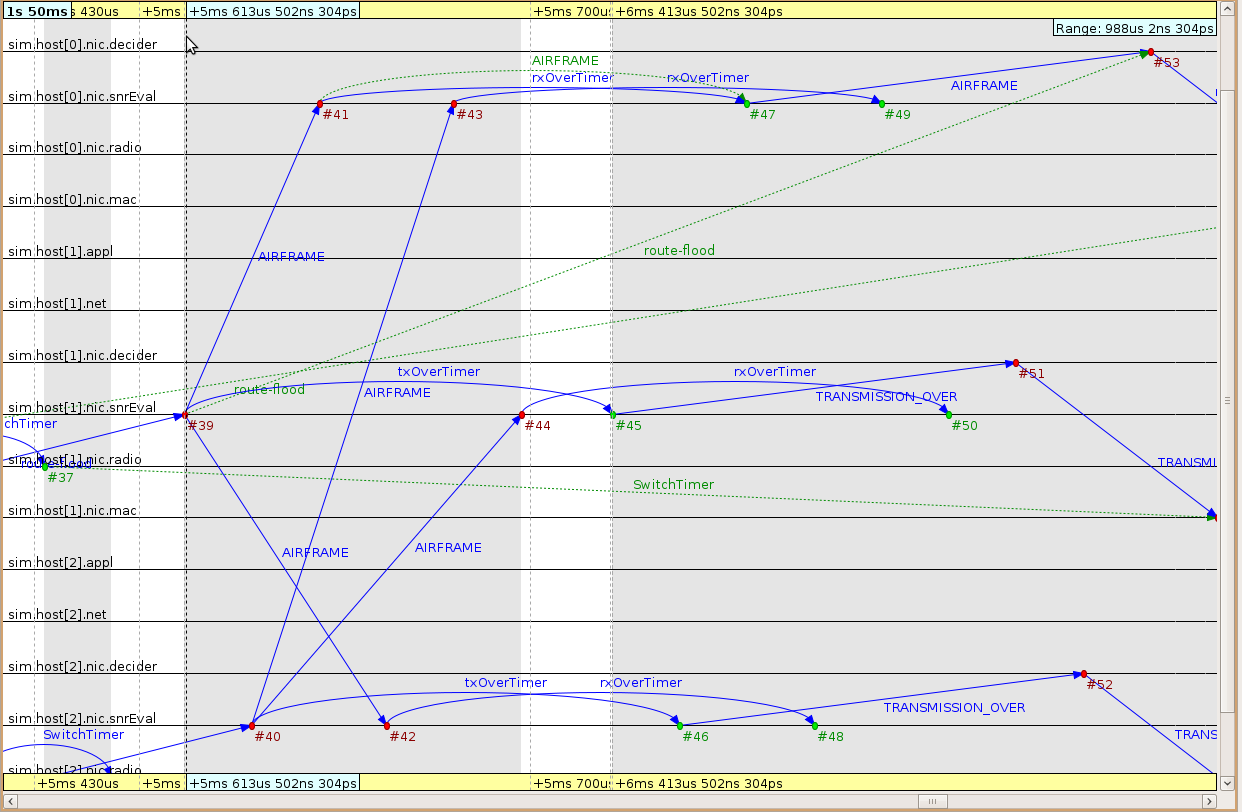
\includegraphics[angle=90, width=15cm]{./figures/kolizia.png}
 % topologies802154.png: 722x407 pixel, 72dpi, 25.47x14.36 cm, bb=0 0 722 407
 \caption{Kolízia na MAC vrstve}
 \label{fig:kolizia}
\end{figure}

%*****************************************************************************
\chapter{Testovanie}

V tejto časti popíšem testy, ktoré som uskutočnil pomocou daného modelu a porovnám výsledky týchto testov s reálnym meraním.

\subsection{Testy zamerané na pohyb XBee zariadení}
Pri vykonávaní týchto testov, som modeloval komunikáciu dvoch XBee zariadení, z ktorých jedno bolo v pozícii príjemcu a vysielač sa pohyboval. Hlavný faktor, na ktorý som kládol dôraz bolo pozorovanie ako sa mení hodnota výkonu na strane príjemcu s narastajúcou vzdialenosťou. Taktiež som sledoval počet zahodených rámcov, takzvanú stratovosť rámcov (na základe výpočtu chybovosti BER na prijímači) s narastajúcou vzdialenosťou a oslabovaním sa signálu, viď tabuľka \ref{tab:stratovost1} \\

Vykonal som následujúce testy:
\begin{enumerate}
 \item vzdiaľovanie sa vysielača (s výkonom vysielača 1mW a 10mW) po kroku 0.6cm (po každom kroku bol vyslaný rámec) do vzdialenosti 5m, viď. grafy \ref{fig:5m-1mW} a \ref{fig:5m-10mW}
 \item vzdiaľovanie sa vysielača (s výkonom vysielania 1mW a 10mW) po kroku 0.6cm (po každom kroku bol vyslaný rámec) do vzdialenosti 5m a súčasná náhodná rotácia oboch zariadení okolo vlastnej osi
 \item vzdiaľovanie sa vysielača (s výkonom vysielania 1mW  a 10mW) po kroku 0.6m (po každom kroku bol vyslaný rámec) do vzdialenosti 250m, viď. graf  \ref{fig:250m-10mW}
 \item vzdiaľovanie sa vysielača (s výkonom vysielania 1mW  a 10mW) po kroku 0.6m (po každom kroku bol vyslaný rámec) do vzdialenosti 250m a súčasná náhodná rotácia oboch zariadení okolo vlastnej osi, viď. graf \ref{fig:250m-1mW-rotace}
 \item náhodná rotácia vysielača okolo prijímača vo fixnej vzdialenosti 10m
\end{enumerate}

Detailné výstupy z týchto testov sa nachádzajú na priloženom CD vo forme spracovaných grafov a taktiež vo forme súboru s príponou .sca, čo je jeden z výstupných formátov simulátoru Omnet, ktorý sa dá ďalej vhodne spracúvať pomocou nástroja Scave.

%Grafy z merani

%Grafy z realu
Analýzou týchto meraní je vidno, že krivky grafov sa takmer zhodujú s reálnymi meraniami a to aj napriek tomu, že reálne prostredie obsahuje množstvo faktorov spôsobujúcich odrazy atď. Daným modelom som schopný modelovať reálne podmienky s vysokou presnosťou aj napriek tomu, že zanedbám straty, ktoré v nich vznikajú.

\begin{table}[htbp]
\begin{center}
\begin{tabular}{|c|c|c|}
\hline Vzdialenosť [m] & Stratovosť [\%] & Výkon vysielača [mW]\\ 
\hline 100 & 0 & 1\\ 
\hline 150 & 0.12 & 1\\ 
\hline 200 & 11.87 & 1\\ 
\hline 220 & 30.42 & 1\\ 
\hline 250 & 76.38 & 1\\
\hline 300 & 49.65 & 10\\  
\hline 
\end{tabular} 
\end{center}
\caption{Stratovosť rámcov}
\label{tab:stratovost1}
\end{table}

\subsection{Testy s kolíziou}
V týchto testoch bola poloha zariadení XBee stacionárna. Model uvažoval dve zariadenia prijímač a vysielač, kde vysielač vysielal rámce. Ďalej som do simulácie zapojil generátor šumu (zariadenie periodicky generujúce rámce, ktoré spôsobovali kolíziu). V tejto simulácii som sledoval koľko rámcov bolo zahodených (stratovosť) z dôvodu šumu spôsobeného generátormi na prijímači. \\

Vykonal som následujúce testy:
\begin{enumerate}
 \item model viď. obrázok \ref{fig:modelKolizie} prijímač - host[0], vysielač - host[1] boli umiestnené vo vzdialenosti 30cm, generátor šumu - host[2] (vysielací výkon 10mW) vo vzdialenosti 3m a 4m
 \item model totožný s predchádzajúcim no bol pridaný druhý generátor šumu, jeho umiestnenie bolo x = host[2].x - 0.7m, y = host[2].y. Vysielací výkon oboch generátorov šumu bol 10mW. 
\end{enumerate}

\begin{table}[htbp]
\begin{center}
\begin{tabular}{|c|c|c|}
\hline Vzdialenosť generátora šumu [m] & Stratovosť [\%] & Stratovosť v reálnych podmienkach [\%]\\ 
\hline 3 & 9.8 &15\\ 
\hline 4 & 0 & nebolo merané\\ 
\hline 
\end{tabular} 
\end{center}
\caption{Prípad č. 1}
\label{tab:stratovost2}
\end{table}

\begin{table}[htbp]
\begin{center}
\begin{tabular}{|c|c|}
\hline Vzdialenosť generátorov šumu [m] & Stratovosť [\%] \\ 
\hline 3 & 98\\ 
\hline 4 & 80\\ 
\hline 
\end{tabular} 
\end{center}
\caption{Prípad č. 2}
\label{tab:stratovost3}
\end{table}
%tabulka


%vyhodnotenie ???

\begin{figure}[htbp]
 \centering
 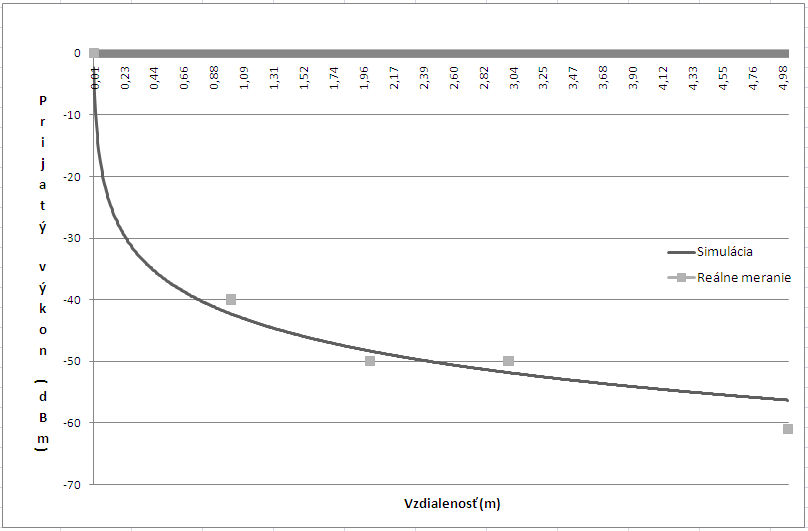
\includegraphics[width=13cm]{./figures/results/5m-1mw.png}
 % topologies802154.png: 722x407 pixel, 72dpi, 25.47x14.36 cm, bb=0 0 722 407
 \caption{Pohyb na vzdialenosť 5m, vysielací výkon 1mW}
 \label{fig:5m-1mW}
\end{figure}

\begin{figure}[htbp]
 \centering
 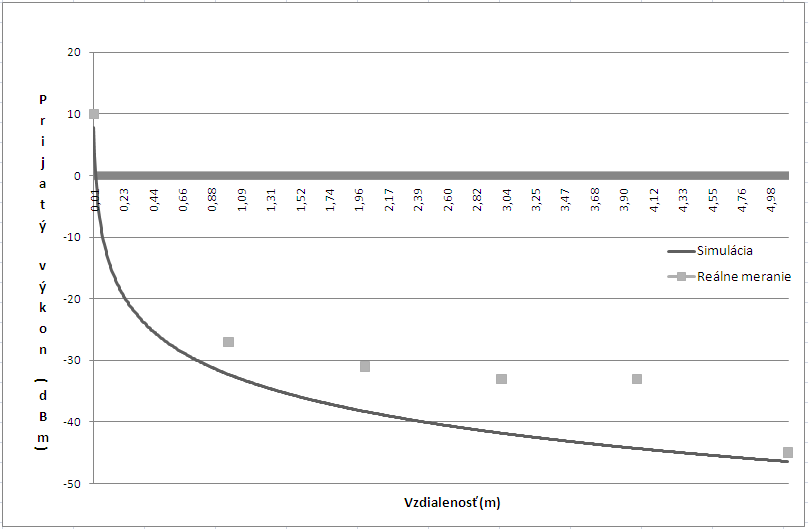
\includegraphics[width=13cm]{./figures/results/5m-10mw.png}
 % topologies802154.png: 722x407 pixel, 72dpi, 25.47x14.36 cm, bb=0 0 722 407
 \caption{Pohyb na vzdialenosť 5m, vysielací výkon 10mW}
 \label{fig:5m-10mW}
\end{figure}

\begin{figure}[htbp]
 \centering
 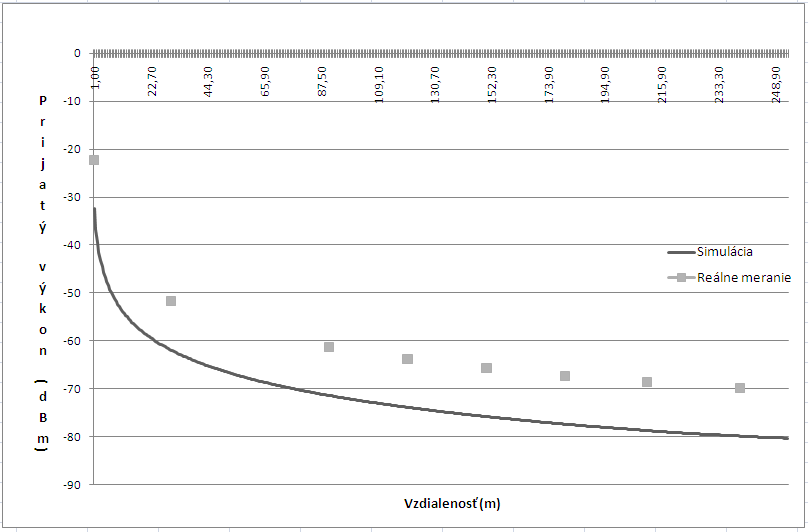
\includegraphics[width=13cm]{./figures/results/250-10mw.png}
 % topologies802154.png: 722x407 pixel, 72dpi, 25.47x14.36 cm, bb=0 0 722 407
 \caption{Pohyb na vzdialenosť 250m, vysielací výkon 10mW}
 \label{fig:250m-10mW}
\end{figure}

\begin{figure}[htbp]
 \centering
 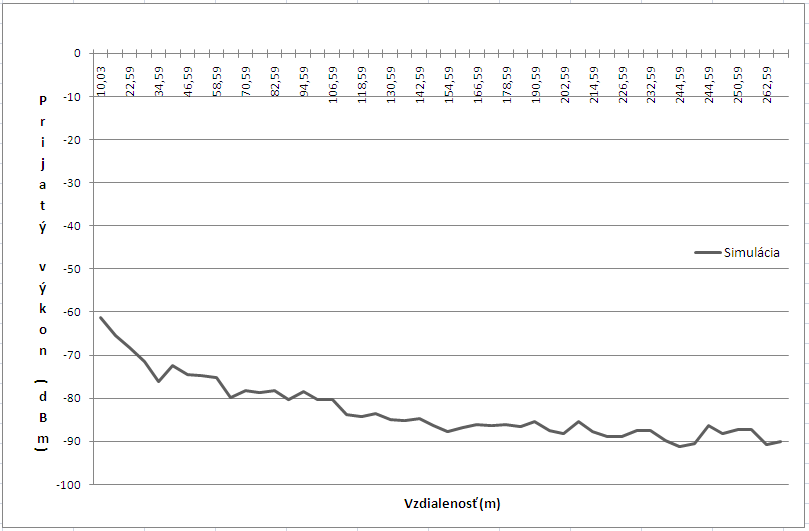
\includegraphics[width=13cm]{./figures/results/250-1mw-rotace.png}
 % topologies802154.png: 722x407 pixel, 72dpi, 25.47x14.36 cm, bb=0 0 722 407
 \caption{Pohyb na vzdialenosť 250m, vysielací výkon 1mW, rotácia okolo vlastnej osi}
 \label{fig:250m-1mW-rotace}
\end{figure}


%*****************************************************************************
\chapter{Záver}




%\item Zhodnocení splnění cílů DP/BP a  vlastního přínosu práce (při formulaci je třeba vzít v potaz zadání práce).
%\item Diskuse dalšího možného pokračování práce.

%*****************************************************************************
% Seznam literatury je v samostatnem souboru reference.bib. Ten
% upravte dle vlastnich potreb, potom zpracujte (a do textu
% zapracujte) pomoci prikazu bibtex a nasledne pdflatex (nebo
% latex). Druhy z nich alespon 2x, aby se poresily odkazy.

\bibliographystyle{abbrv}
%bibliographystyle{plain}
%\bibliographystyle{psc}
{
%JZ: 11.12.2008 Kdo chce mit v techto ukazkovych odkazech take odkaz na CSTeX:
\def\CS{$\cal C\kern-0.1667em\lower.5ex\hbox{$\cal S$}\kern-0.075em $}
\bibliography{reference}
}

% M. Dušek radi:
%\bibliographystyle{alpha}
% kdy citace ma tvar [AutorRok] (napriklad [Cook97]). Sice to asi neni  podle ceske normy (BTW BibTeX stejne neodpovida ceske norme), ale je to nejprehlednejsi.
% 3.5.2009 JZ polemizuje: BibTeX neobvinujte, napiste a poskytnete nam styl (.bst) splnujici citacni normu CSN/ISO.

%*****************************************************************************
%*****************************************************************************
\appendix


%*****************************************************************************
\chapter{Zoznam použitých skratiek}

\begin{description}
\item[APL] Aplication Layer
\item[APS] Aplication Support Sub-layer
\item[CSMA-CA] Carrier Sense Multiple Access - Collision Avoidance
\item[FFD] Full Functionality DEvice
\item[FEL] Future Event List
\item[FES] Future Event Set
\item[FSPL] Free-space path loss
\item[GTS] Guaranteed Time Slot
\item[GUI] Graphical User Interface
\item[IDE] Integrated Development Environment
\item[LQI] Link Quality Indicator
\item[LR-WPAN] Low-Rate Wireless Personal Area Network
\item[MAC] Medium Access Control
\item[MF] Mobility Framework
\item[NED] Network Description
\item[NIC] Network Card Interface
\item[NWK] Network
\item[RFD] Reduced Functionality Device
\item[PAN] Person Area Network
\item[PHY] Physical
\item[SAP] Service Access Point
\item[SFD] Start Frame Delimiter
\item[SNR] Signal to noise ratio
\item[ZDO] ZigBee Device Object
\item[WLAN] Wireless Local Area Network
\item[WPAN] Wireless Personal Area Network
\end{description}


%*****************************************************************************
\chapter{Inštalačná a užívateľská príručka}

\subsection{Inštalácia simulátoru OMNeT++ pre platformu Linux}
\begin{enumerate}
 \item Stiahnutie archívu obsahujúceho zdrojový kód zo stránok \\
 \url{http://www.omnetpp.org/omnetpp}
 \item Prekopírovanie archívu do adresára /usr/local/
 \item Rozbalenie archívu pomocou príkazu tar zxvf omnetpp-4.0.src.tgz
 \item Do užívateľského profilu .bash\_profile alebo .profile pridáme riadok \\
  export PATH=\$PATH:/usr/local/omnetpp-4.0/bin
  \item Je potreba zabezpečiť prítomnosť následujúcich balíkov v systéme 
    \begin{tabbing}
    sudo apt-get install \= build-essential gcc g++ bison flex perl tcl8.4 tcl8.4-dev \\
                       \> tk8.4 tk8.4-dev blt blt-dev libxml2 libxml2-dev \\
                       \> zlib1g zlib1g-dev libx11-dev
    \end{tabbing}    
 \item Prevedieme následujúce príkazy: \\
   cd /usr/local/ometpp-4.0 \\
   ./configure \\
   ./make
 \item Spustenie OMNeT++ s IDE pomocou príkazu omnetpp 
\end{enumerate}

\subsection{Inštalácia mnou modifikovaného Mobility Frameworku}
\begin{enumerate}
 \item Stiahnutie súborov Mobility frameworku z svn http://my-svn.assembla.com/svn/mframework/, poprípade prekopírovanie adresára mf2o4 z priloženého CD do adresára /usr/local/
 \item Import MF do aplikácie OMNeT++
  \begin{enumerate}
   \item Po spustení aplikácie Omnet, klikneme na oblasť \uv{Project explorer}, pravým tlačítkom a zvolíme položku \uv{Import...}
   \item Zvolíme \uv{General->Existing project into Workspace}
   \item V položke \uv{Select root directory}, zvolíme cestu k adresáru mf2o4, tj. /usr/local/mf2o4
   \item Pomocou CTRL+B, preložíme zdrojové súbory
  \end{enumerate}  
\end{enumerate}

\subsection{Práca s modelom IEEE 802.15.4}
Vo vývojom prostredí Omnetu si otvoríme v oblasti \uv{Project explorer} adresárovú štruktúru mf2o4, kde si následne otvoríme adresár networks a v ňom adresár ieee802.15.4. V tomto adresári sa nachádzajú aj xml súbory popisujúce antény. Otvoríme si súbor omnetpp.ini, tento súbor je hlavným konfiguračným súborom modelu simulácie. Zahrnul som do neho ukážkové nastavenia viacerých modelov, ktoré som simuloval. Samotná simulácia sa potom spustí otvorením súboru omnetpp.ini a následným kliknutím na tlačítko \uv{Run} z menu aplikácie.

%*****************************************************************************
\chapter{Obsah priloženého CD}

Následujúci obrázok \ref{fig:zoznamCD} zobrazuje štruktúru priloženého CD.

\begin{figure}[h]
\begin{center}
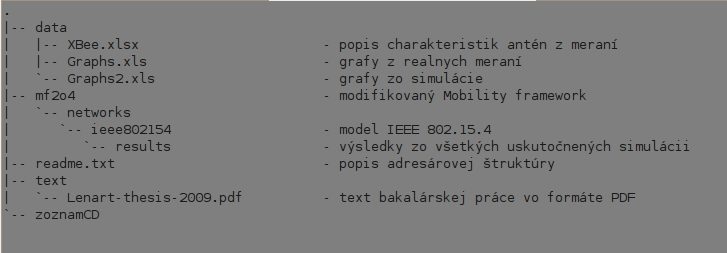
\includegraphics[width=14cm]{./figures/zoznamCD.png}
\caption{Výpis priloženého CD}
\label{fig:zoznamCD}
\end{center}
\end{figure}

\end{document}
